\documentclass[conference]{IEEEtran}
\IEEEoverridecommandlockouts
% The preceding line is only needed to identify funding in the first footnote. If that is unneeded, please comment it out.
\usepackage{cite}
\usepackage{amsmath,amssymb,amsfonts}
\usepackage{algorithmic}
\usepackage{subcaption}
\usepackage{graphicx}
\usepackage{textcomp}
\usepackage{xcolor}
\usepackage{multirow}
\usepackage[numbers]{natbib}       % For bibliography; use numeric citations
\bibliographystyle{IEEEtran}
\def\BibTeX{{\rm B\kern-.05em{\sc i\kern-.025em b}\kern-.08em
    T\kern-.1667em\lower.7ex\hbox{E}\kern-.125emX}}
\begin{document}

\makeatletter
\newcommand{\linebreakand}{%
  \end{@IEEEauthorhalign}
  \hfill\mbox{}\par
  \mbox{}\hfill\begin{@IEEEauthorhalign}
}
\makeatother
\graphicspath{{images/}}

\title{Improving Pose Estimation on Art Collections with Style Transfer}

\author{\IEEEauthorblockN{Tristan Verheecke}
\IEEEauthorblockA{\textit{Ghent University}\\
Ghent, Belgium \\
tristan.verheecke@ugent.be}
\and
\IEEEauthorblockN{Dieter De Witte}
\IEEEauthorblockA{\textit{IDLab, Ghent University}\\
Ghent, Belgium \\
dieter.dewitte@ugent.be}
\and
\IEEEauthorblockN{Steven Verstockt}
\IEEEauthorblockA{\textit{IDLab, Ghent University}\\
Ghent, Belgium \\
steven.verstockt@ugent.be}
\linebreakand
\IEEEauthorblockN{Kenzo Milleville}
\IEEEauthorblockA{\textit{IDLab, Ghent University}\\
Ghent, Belgium \\
kenzo.milleville@ugent.be}
\and
\IEEEauthorblockN{Ravi Kharti}
\IEEEauthorblockA{\textit{IDLab, Ghent University}\\
Ghent, Belgium \\
ravi.khatri@ugent.be}
}

\maketitle

\begin{abstract}
Through digitalization, museums are given the ability to more efficiently analyze their art collections.
Important connections between artworks can be uncovered this way, which can be useful for classification or retrieval.
Museums put a great amount of effort in this process, but it can be very labor intensive doing this manually.
To eliminate this issue, they've sought to automate these tasks using computer vision methods.
In computer vision, there's a rich volume of research in image classification, semantic segmentation, object detection and 2D/3D human pose estimation (HPE).
It turns out however, that these algorithms aren't suitable for tasks on art collections as they were trained on photographs.
This paper will deal with the HPE problem and what methods can be used to improve performance on art collections.
Two shortcomings can be identified: incomplete keypoint prediction and wrong pose association.
To solve this problem, this paper proposes a method which fine-tunes state-of-the-art (SOTA) HPE models with a combination of stylized COCO datasets.
Three datasets were created from the WikiArt dataset representing baroque, renaissance and impressionism.
From those genres a selection of figurative paintings is made using content-based image retrieval.
Then for each style transfer model, first, a mixture of genres is used and, second, one with only impressionism to create a stylized COCO dataset.
This is done for CycleGAN and AdaIN.
Then, the SWAHR and ViTPose pose estimation models are fine-tuned on the COCO dataset in combination with the stylized COCO dataset and with only the stylized COCO dataset.
This makes a total of 16 models that are evaluated and in which a consistent improvement in pose estimation prediction was found.
\end{abstract}

\begin{IEEEkeywords}
Cultural Heritage, Computer Vision, Deep Learning, 2D Human Pose Estimation, Style Transfer, CycleGAN, AdaIN, SWAHR, ViTPose
\end{IEEEkeywords}

\section{Introduction}
Part of the modern age is the digitalization of information.
Digitization makes information more accessible to a broader audience and allows it to be processed more efficiently.
Museums have put huge efforts in digitalizing their catalogue as well, as this can help in Iconography; this is the branch of art history that concerns itself with the themes and motifs of artworks.
Through the analysis of artworks, different connections between different artworks can be established, which can be useful for classification or retrieval.
However, art collections don't contain much metadata and it is time-consuming to enhance them manually.
Museums want to utilize computer vision to automate this process, but the algorithms that were developed over the last few decades, are mainly for photography and it turns out that art collections (paintings, statues, drawing, etc) are less interpretable by these algorithms.

Computer vision can perform a wide range of tasks, including image classification, semantic segmentation, object detection, and 2D/3D human pose estimation (HPE).
For this paper, the focus will be on 2D HPE.
A database can be created with the different poses found in the artworks which can be used to discover similar themes and categorize them.
There is an extensive amount of research based around HPE that can be useful for this.

To make the vast quantity of research around HPE available to art collections, the following proposed solution will be explored:
If the pre-trained models can't be used, it's still an option to retrain one with an augmented dataset.
With style transfer the images of existing datasets can be stylized and added to the datasets.
This will increase the size and variance of the dataset, making it better to train on.
This can increase performance on art collections as stylized images are also being trained on but can also potentially increase the performance on photographs.

\section{Related Work}
\subsection{Generative Adversarial Network}
Proposed by Goodfellow et al. \cite{Goodfellow2014}, a Generative Adversarial Network (GAN) is a framework where a generative model competes against a discriminative model.
It consists of a generator $G$ which takes in random noise and attempts to output a sample from a specific distribution, while the discriminator $D$ will try to distinguish between the sample from the generator and a real sample from that distribution.
A popular variation of GAN is the conditional GAN, this architecture feeds an extra label to the generator and discriminator, so that it can be conditioned to generate certain images based on the label.

\subsection{Human Pose Estimation}
Human Pose Estimation (HPE) aims to detect human features from input data such as images and videos.
It's an elementary part of computer vision with many applications among which are: human action recognition (sign language), human tracking (surveillance), and human-computer interaction (video games).
This is an extensively researched area with a diverse range of different techniques.
The human body has a high degree-of-freedom due to all the limbs, self-similar parts and body types, which may cause self-occlusion or rare/complex poses.
The variations in configuration are made even larger due to clothing, lighting, foreground occlusion, as well as viewing angles and truncation, among others.
This makes HPE one of the most difficult tasks in computer vision.

\subsubsection{Single-Person Human Pose Estimation}
\textbf{Heatmap and Detection-based Methods} predict the individual body parts using heatmaps.
This method results in an easier optimization and a more robust generalization \cite{chen2022}.
Most of the latest HPE methods use heatmaps because of this.
After the joints are found, they are assembled to fit a human skeleton, as shown in Figure \ref{fig:single_pose_estimation_heatmap-based_methods}.

\begin{figure}[h]
	\centering
	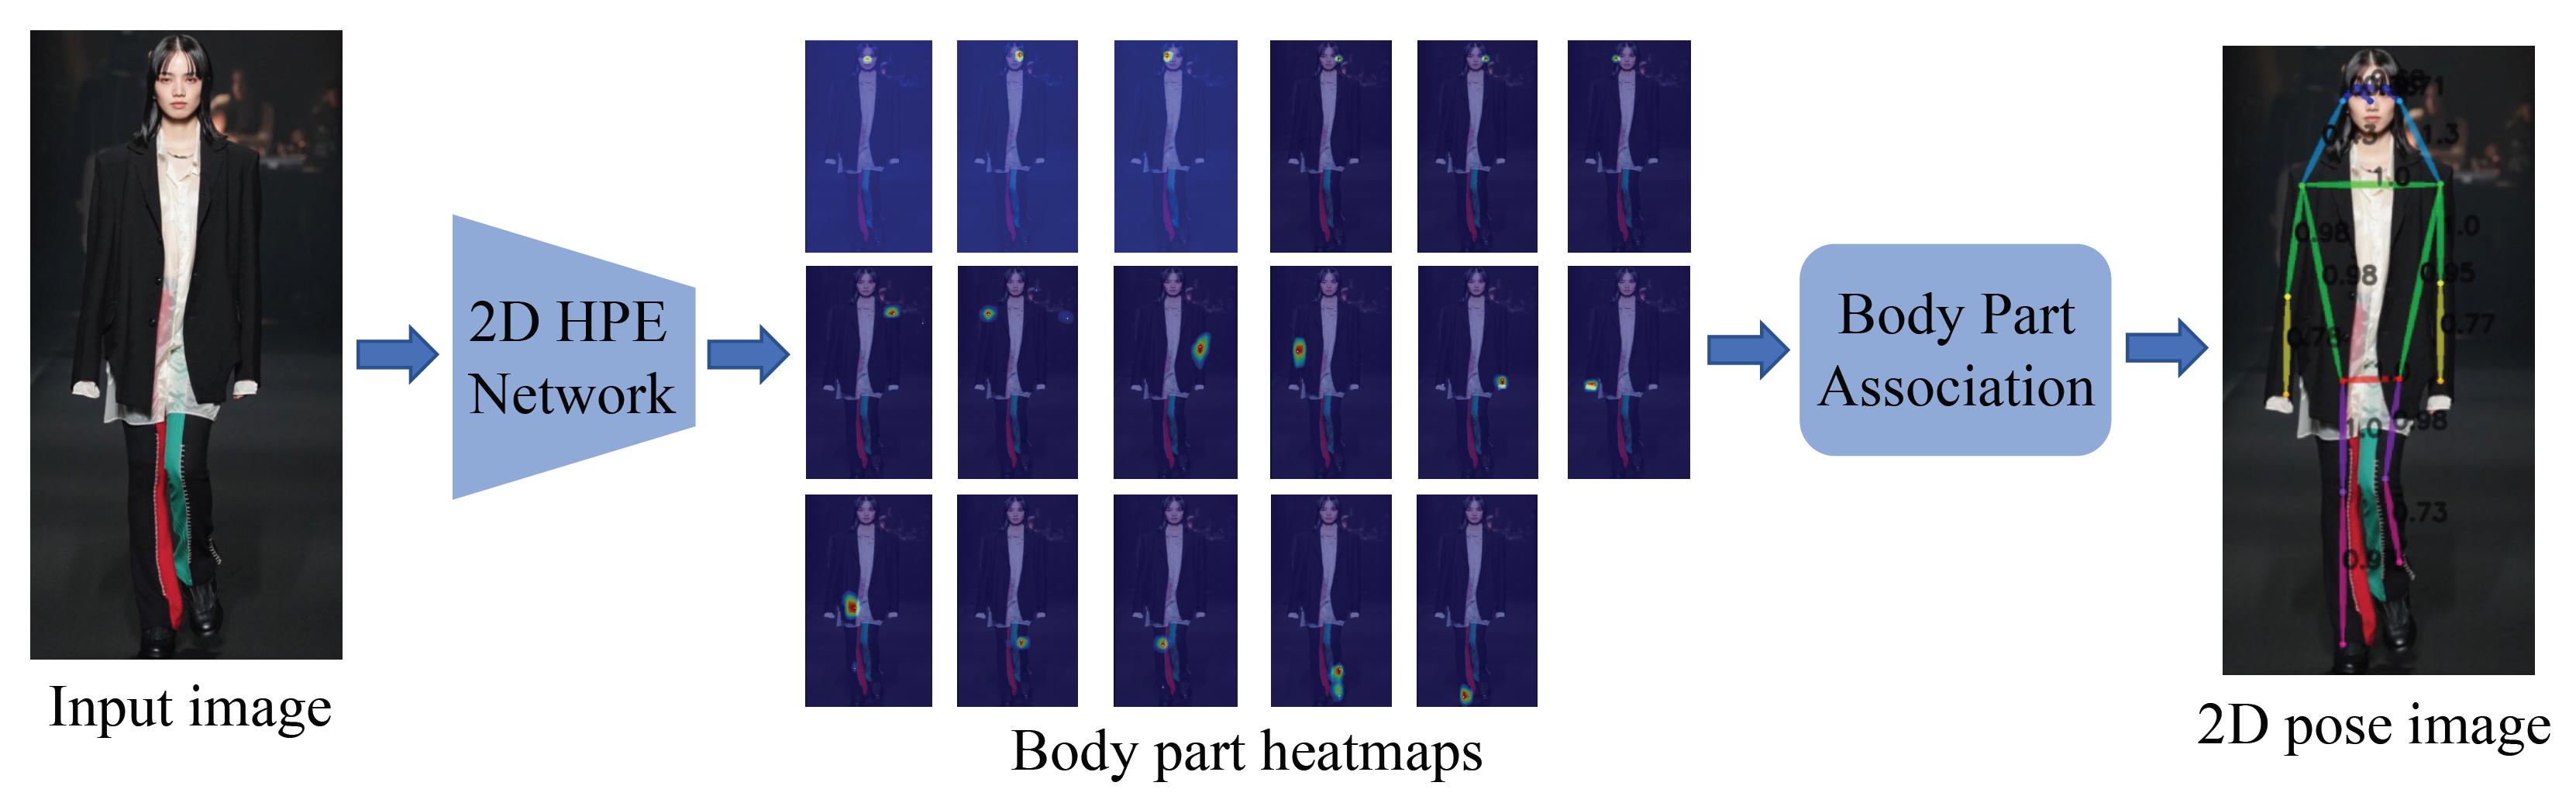
\includegraphics[width=0.48\textwidth]{single_pose_estimation_heatmap-based_methods}%
	\caption{Heatmap-based Methods as presented in \cite{Zheng2012}}
	\label{fig:single_pose_estimation_heatmap-based_methods}
\end{figure}

A fundamental work written by Wei et al. \cite{Wei2016} combines convolution networks with Pose Machines \cite{Ramakrishna2014}.
Pose Machines is an iterative architecture which consists of two models:
The first is used for stage one where it predicts potential heatmaps for the joints.
The second model is used for subsequent stages where the result of the previous stage is fed in together with the results of its own convolution network on the input image. 
This gradually refines the predictions for the joints and their positioning.
Another influential work was being written at the same time by Newell et al. \cite{Newell2016}.
Similar to CPMs, this is also an iterative architecture.
They suggest what they call a "stacked hourglass" network, where "hourglass" modules are repeated.
In an "hourglass" module, first, the features are downsampled and, afterwards, upsampled again.
This network captures different spatial relationships between joints at different resolutions.
Both use intermediate supervision to tackle the problem of vanishing gradients.
This still doesn't build a deep sub-network for feature extraction which limits the predictions.
This has become less of a problem with the emergence of the ResNet \cite{He2015} which allows better back-propagation at deeper levels through shortcuts.
A more recent work by Sun et al. \cite{Sun2019} maintains high-resolution representations instead of working with the high-resolution from the low-to-high sub-network.
After a first high-resolution sub-network, it gradually adds high-to-low sub-networks in parallel to predict multi-resolution features.
Before each branch, they apply multi-scale fusion, which joins the predicted features from each scale on each other scale (Figure \ref{fig:HRNet}).

\begin{figure}[h]
	\centering
	\subcaptionbox{HRNet \label{fig:single_pose_estimation_HRNet}}[0.48\textwidth]{%
		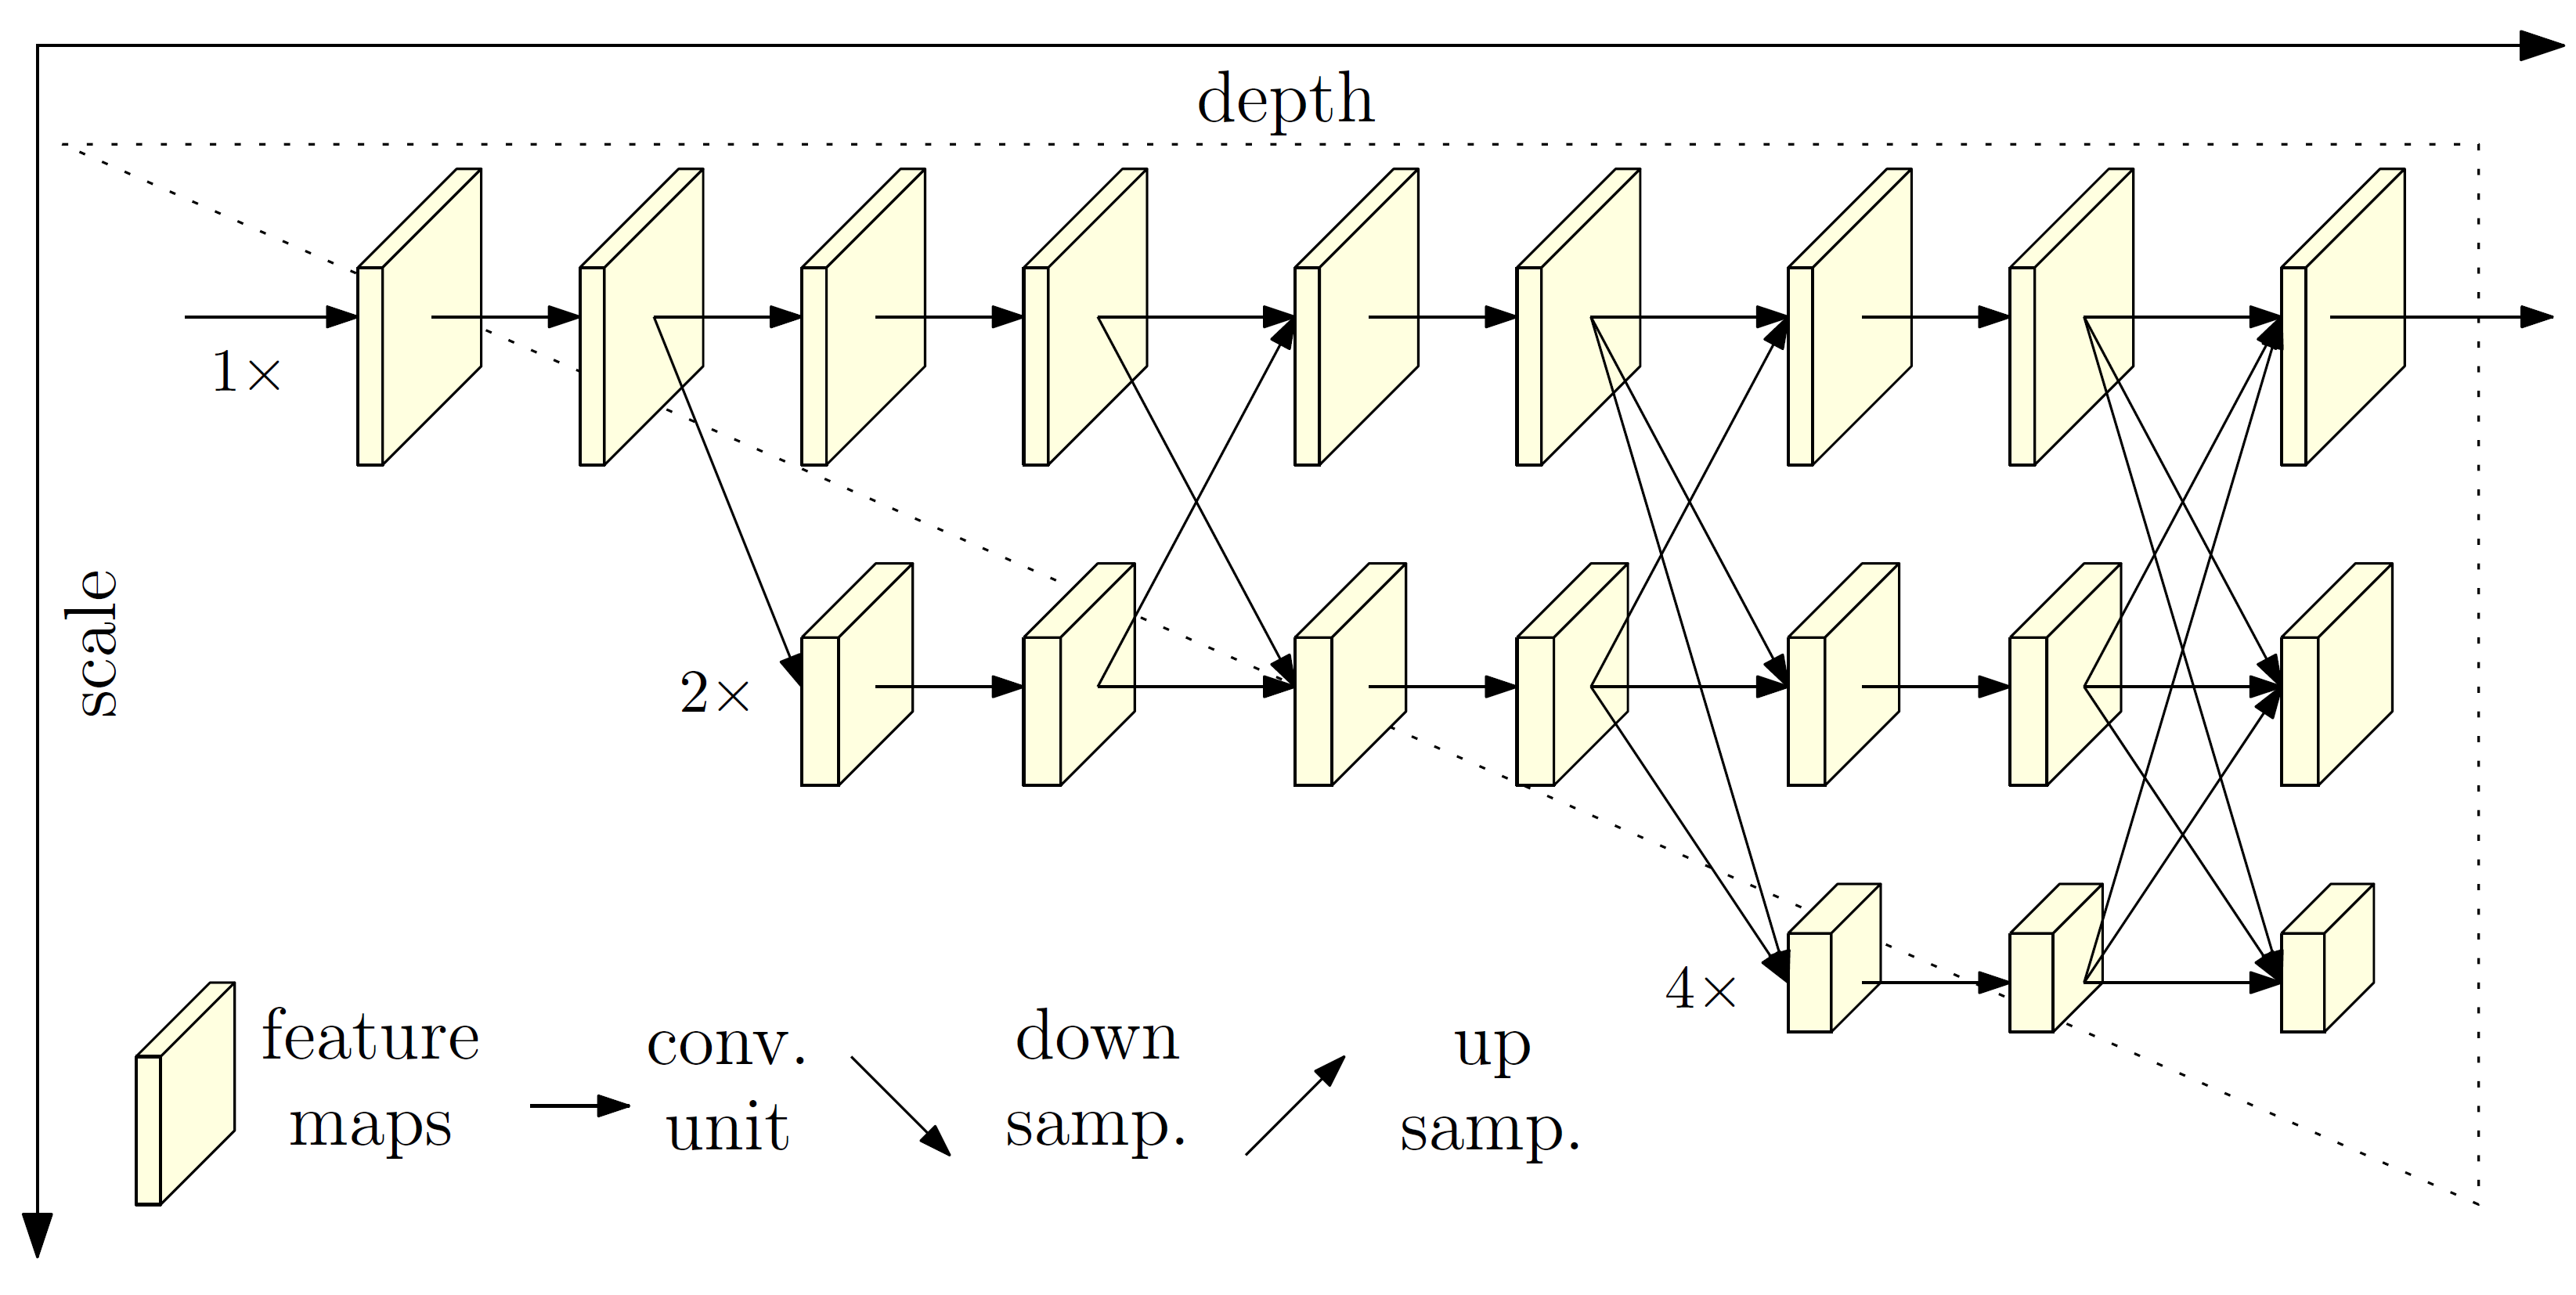
\includegraphics[width=0.48\textwidth]{single_pose_estimation_HRNet}%
	}
	\subcaptionbox{Multi-Scale Fusion \label{fig:single_pose_estimation_multi-scale_fusion}}[0.48\textwidth]{%
		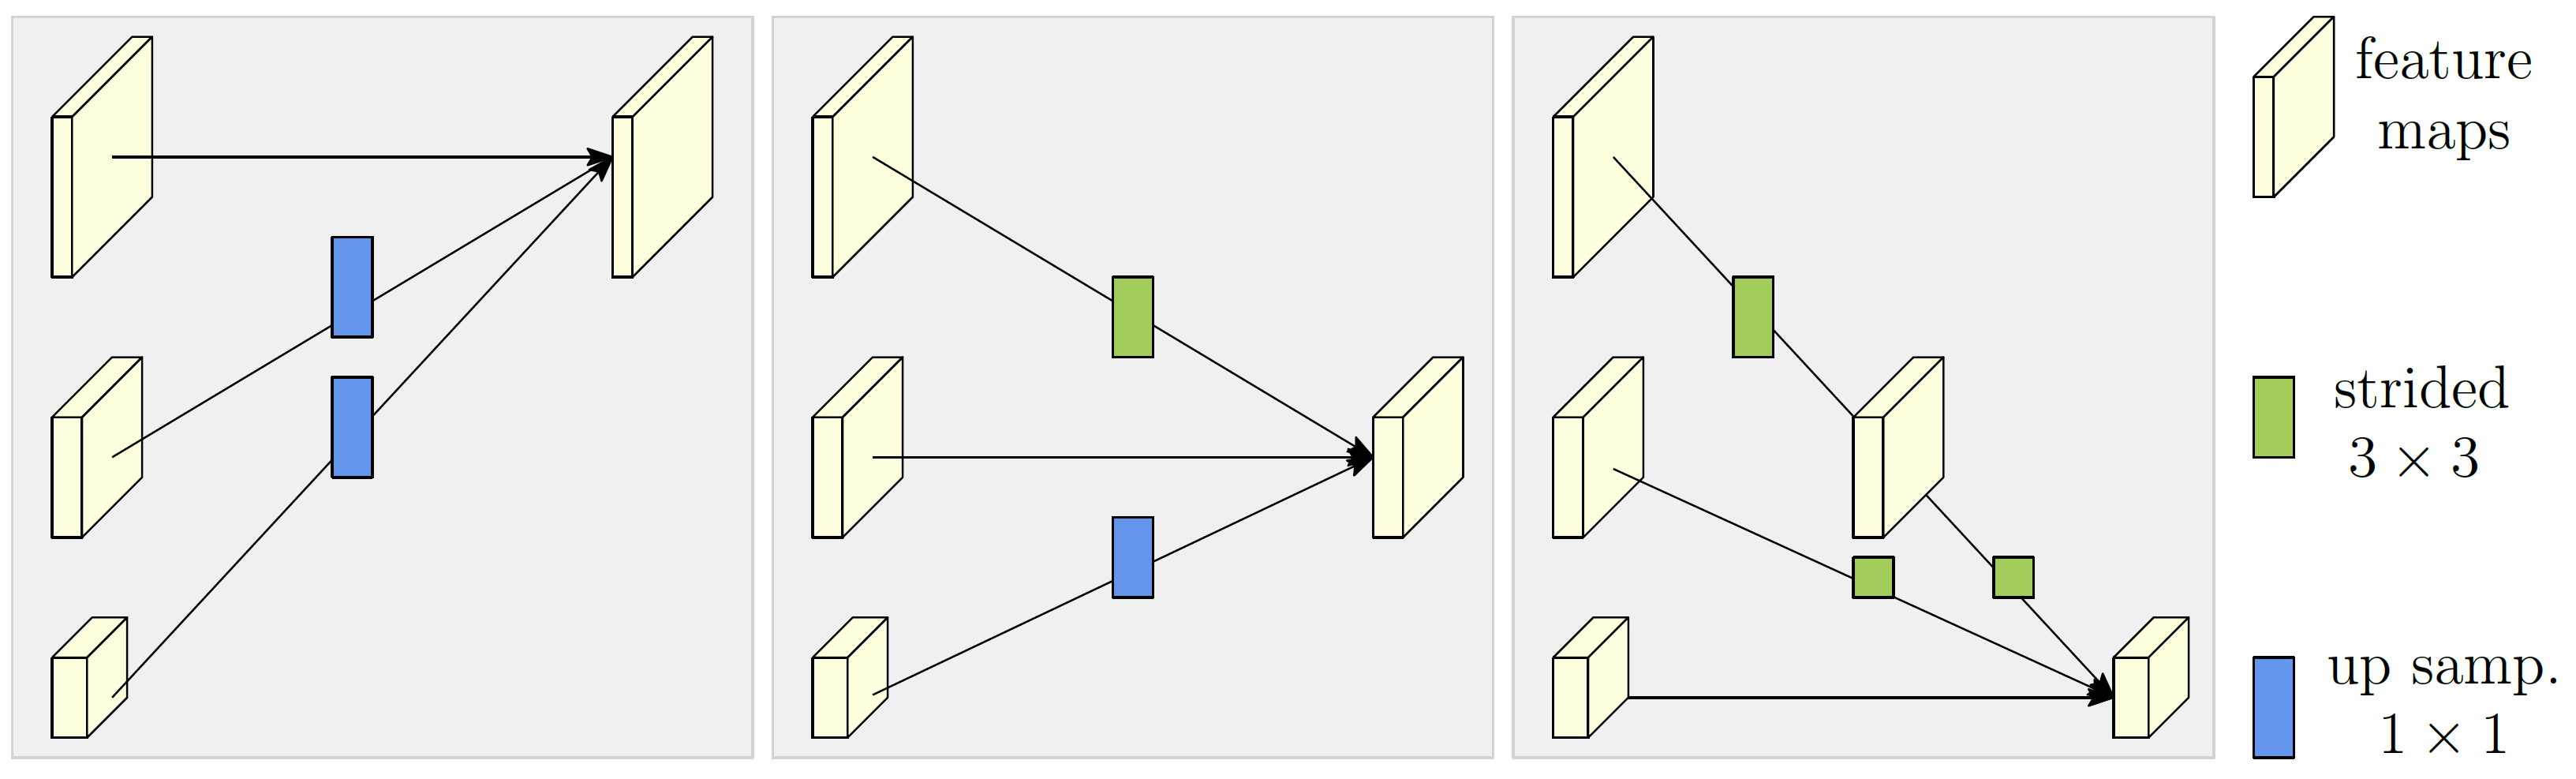
\includegraphics[width=0.48\textwidth]{single_pose_estimation_multi-scale_fusion}%
	}
	\caption{
		The architecture of the High-Resolution network and how it applies multi-scale fusion \cite{Sun2019}.
	}
	\label{fig:HRNet}
\end{figure}

\subsubsection{Multi-Person Human Pose Estimation}
\textbf{Top-Down Human Pose Estimation} will first try to detect all persons in the image with a human detector.
Each person is cropped by the bounding box and single-person HPE predicts a pose.
Iqbal et al. \cite{Iqbal2016} use Faster R-CNN \cite{Ren2015} to detect the human boundaries, after which it applies integer linear programming on each person's fully connected graph to obtain the final pose estimates.
The use of a human detector comes with its own set of problems, which Fang et al. \cite{Fang2016} try to remedy with Regional Multi-person Pose Estimation.
They try to tackle inaccurate bounding boxes with a Symmetric Spatial Transformer Network and redundant detections with Parametric Pose Non-Maximum-Suppresion.
Papandreou et al. \cite{Papandreou2017} use a two stage pipeline, where they, first, employ the Faster R-CNN detector and, second, estimate the pose in each found bounding box using their own network.
It predicts heatmaps using a fully convolutional ResNet and then uses a heatmap-offset aggregation procedure.
Afterwards, they do post-processing using keypoint-based Non-Maximum-Suppression.
A continuous effort is taken by Chen et al. \cite{Chen2017a} to deal with occlusion and truncation.
They suggest a two stage architecture, where, the "simple" keypoints are captured with GlobalNet, a feature pyramid network based on \cite{Lin2016}, and the "hard" keypoints are handled by their RefineNet.
It integrates the information via upsampling and concatenating of HyperNet \cite{Kong2016}, using an adapted stacked hourglass.
In more recent research, a new method was become competitive with CNNs.
Based on work in language modeling, attention mechanisms, an optimization of recurrent networks, allow the modeling of dependencies without regard of the distance in the input or output sequences.
The Transformer, introduced by Vaswani et al. \cite{Vaswani2017}, eliminates recurrence and relies solely on attention mechanisms.
This enables it to work better in parallel, while it still maintains state-of-the-art performance.
Based on this new architecture, Dosovitskiy et al. \cite{Dosovitskiy2020} created a new model that can work with images; the Visual Transformer (ViT).
Xu et al. \cite{xu2022} use ViT to apply it to the HPE task.
It works by splitting the input image into fixed-size patches which are linearly embedded and then fed into the transformer blocks.
The output of this is then processed by different decoders to form the heatmaps.

\begin{figure}[h]
	\centering
	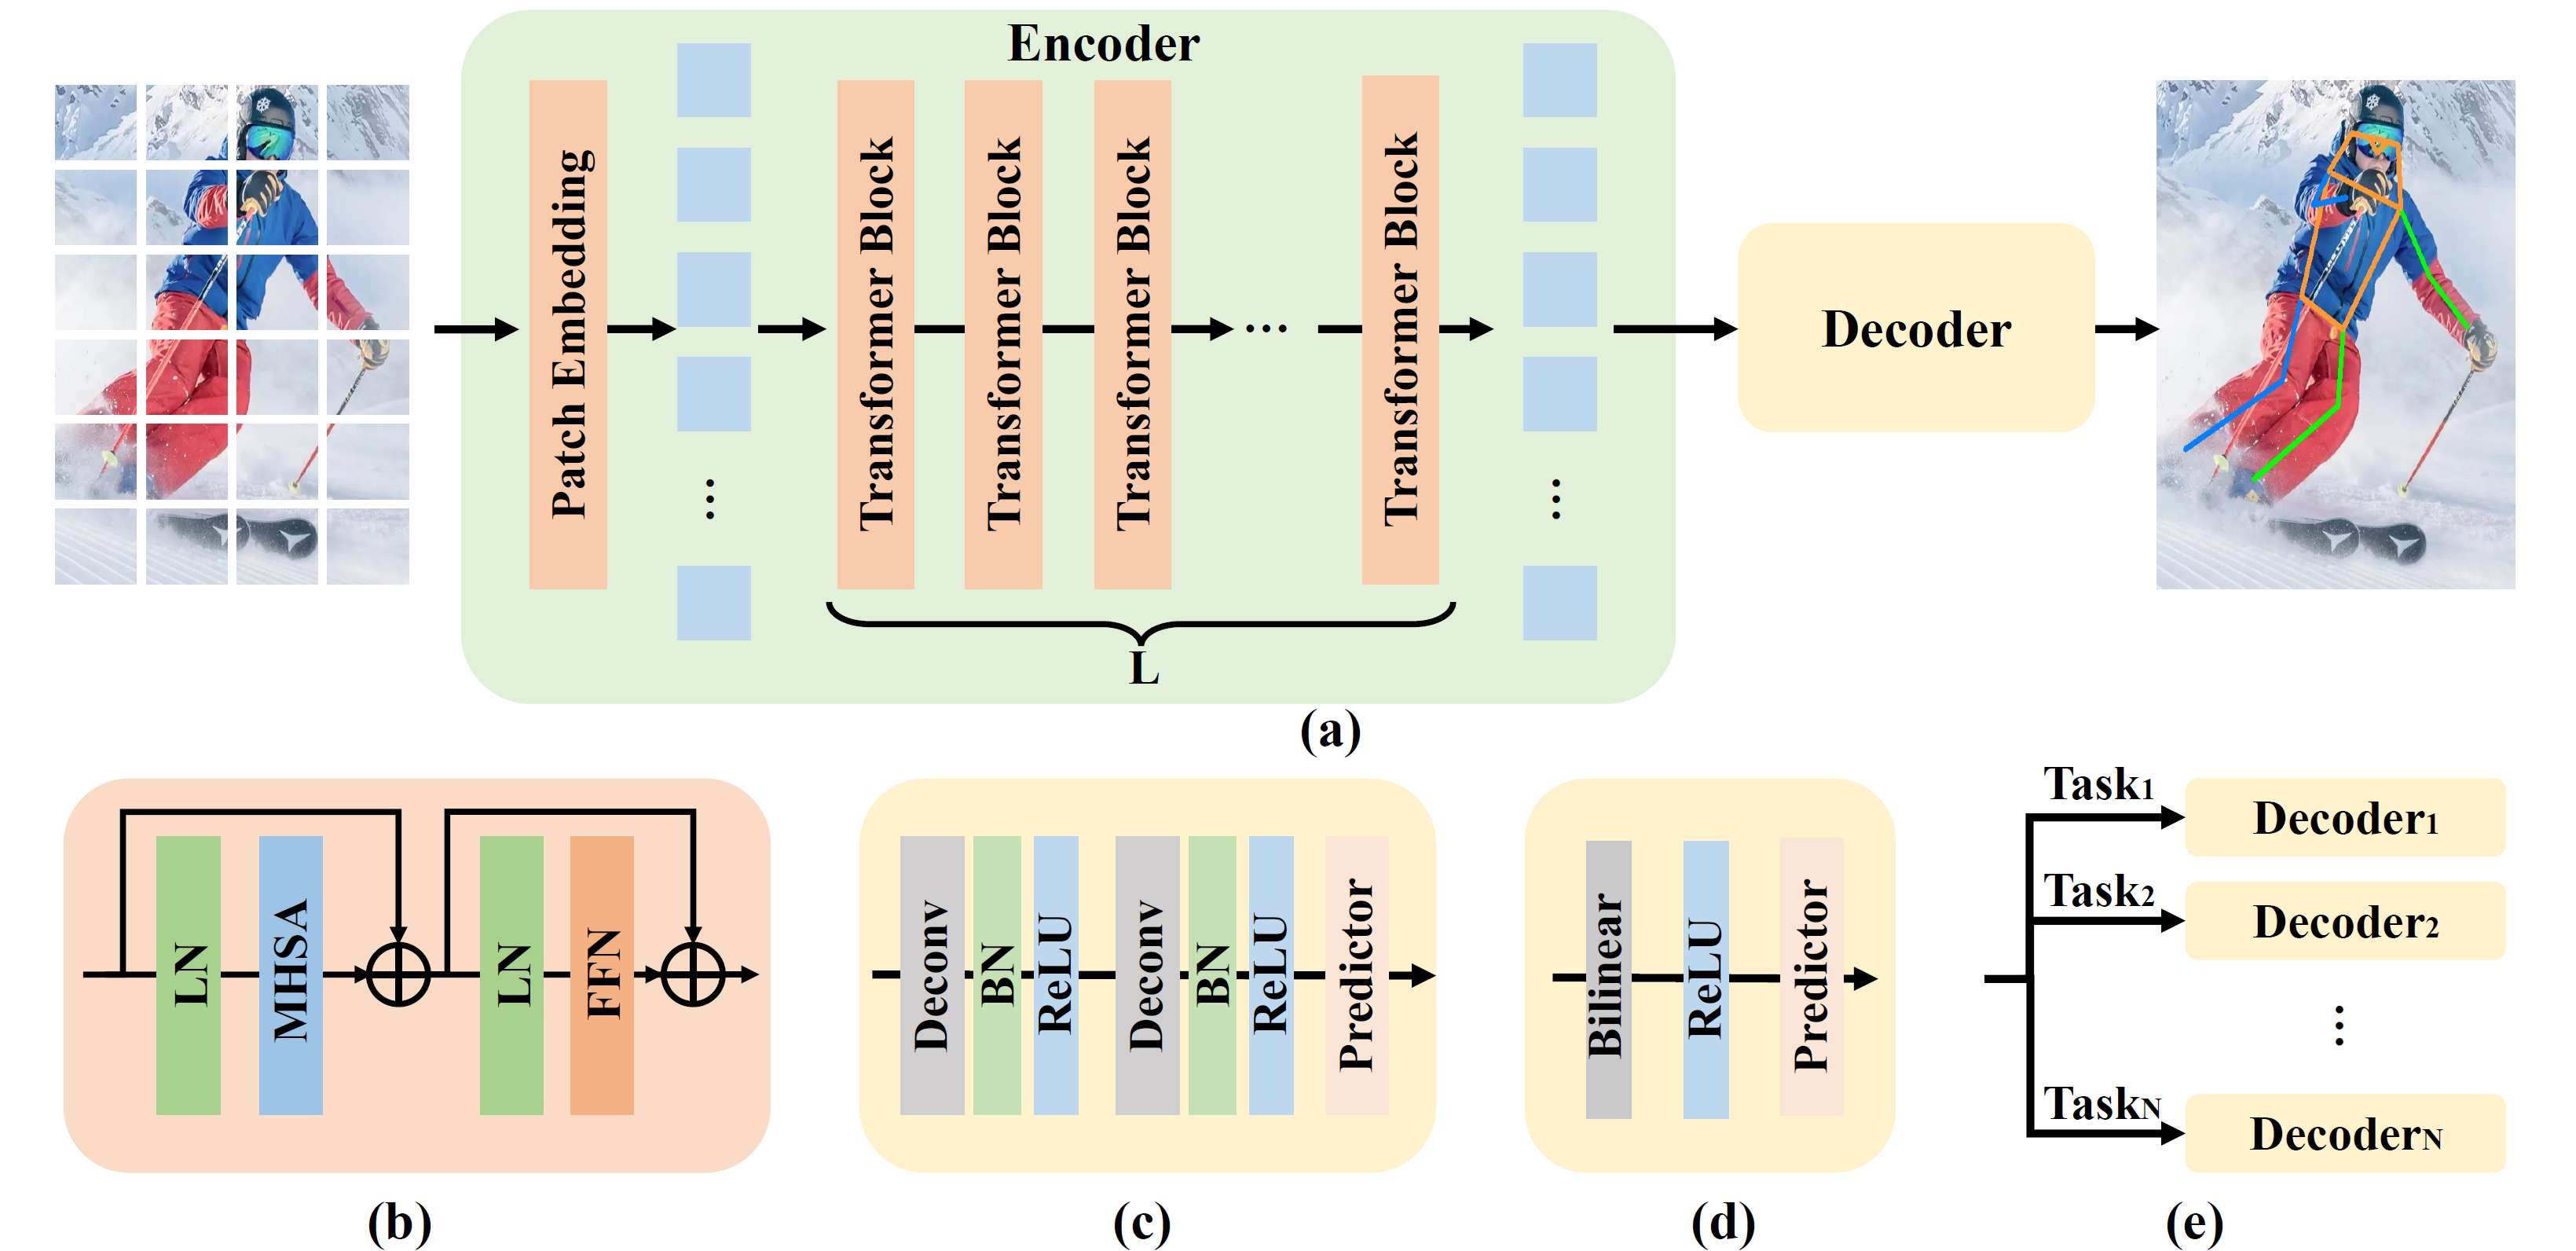
\includegraphics[width=0.48\textwidth]{vitpose}%
	\caption{
		(a) The framework of ViTPose. (b) The transformer block. (c) The classic decoder. (d) The simple decoder. (e) The decoders for multiple datasets. \cite{xu2022}
	}
	\label{fig:vitpose}
\end{figure}

\textbf{Bottom-Up Human Pose Estimation} first locates all joints in the image and then afterwards assemble them in potential poses.
DeepCut by Pishchulin et al. \cite{Pishchulin2015}, uses Fast R-CNN \cite{Ren2015}, it detects the body parts and labels each.
With the joints found, it then uses Integer Linear Programming to assemble them.
However, this method is very computationally expensive.
Insafutdinov et al. \cite{Insafutdinov2016} therefor introduce a stronger part detector and better optimization strategy with DeeperCut.
Convolutional Pose Machines make a return with OpenPose by Cao et al. \cite{Cao2018}.
They're used to predict the joints with heatmaps and Part Affinity Fields, which also encodes the position and orientation of the limb which makes the assembly more reliable.
Kreiss et al. \cite{Kreiss2019} continue on the idea of fields and introduce the Part Association Fields (PIF) and Part Intensity Fields (PAF).
First, they predict the location of the different joints with PIF.
Afterwards, they use PAF to find the inter-joint relationships.
They are able to outperform any previous OpenPose-based proposals on low-resolution and occlusions.
Newell et al. \cite{Newell2016-2} introduce associative embedding.
They make use of the stacked hourglass network from \cite{Newell2016} with some small modifications, and produce joint heatmaps and associative embedding tags.
Continuing on the idea of associative embedding, Cheng et al. \cite{Cheng2019} use HRNet \cite{Sun2019} as backbone for their HigherHRNet (Figure \ref{fig:higherhrnet}).
Their method focuses on the scale-variance problem, so it can localize keypoints for small persons better.
Lou et al. \cite{Lou2020} introduce Scale-adaptive Heatmap Regression and Weight-adaptive Heatmap Regression to the scale-variance problem.
SAHR adaptively adjusts the standard deviation of each heatmap corresponding with the scale of the person.
WAHR rebalances the foreground and background samples, so SAHR can work to its fullest extent.

\begin{figure}[h]
	\centering
	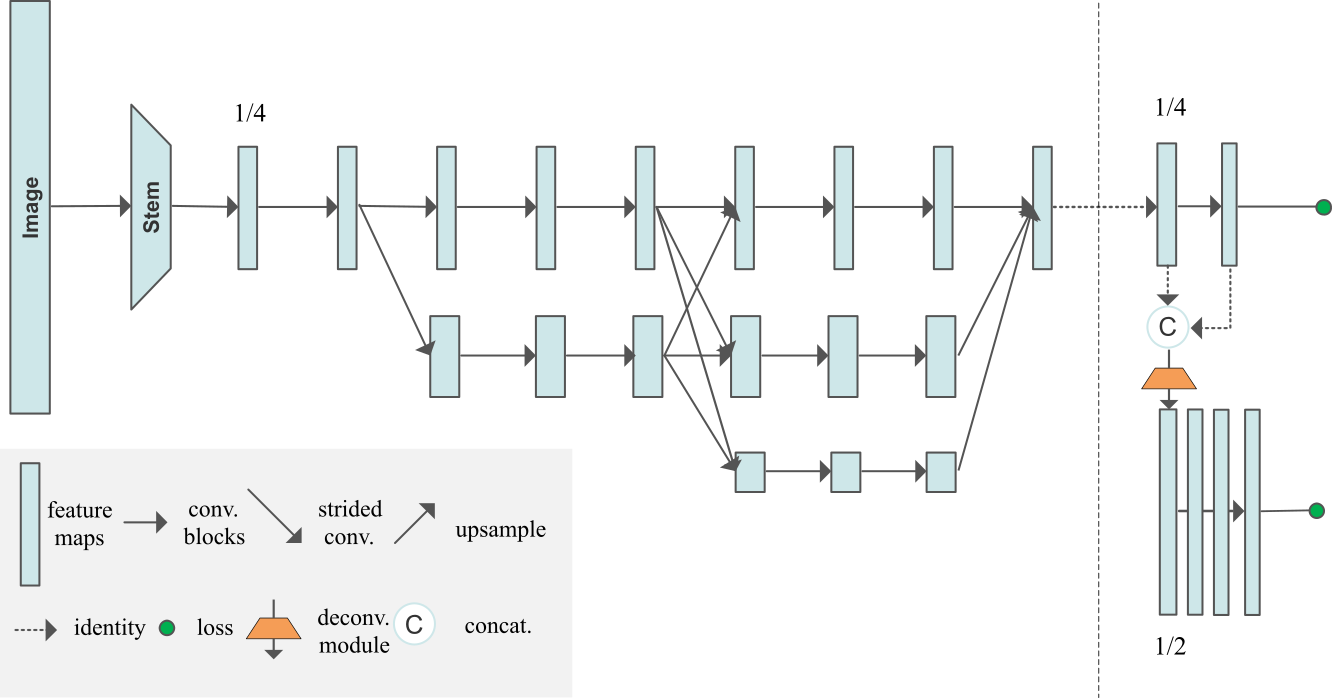
\includegraphics[width=0.48\textwidth]{higherhrnet}%
	\caption{
		The architecture of HigherHRNet. It uses HRNet as backbone. \cite{Cheng2019}
	}
	\label{fig:higherhrnet}
\end{figure}

\subsection{Image Style Transfer}
Image Style Transfer is the technique of applying the style of one image to the content of another.
Traditionally, this is a problem reserved for only artists, but more recently this has also interested computer scientists.
There are several different ideas on how this can be achieved, ranging from how to separate the style from the content to how well an algorithm can generalize.

\subsubsection{Optimization-based Networks}
Gatys et al. \cite{Gatys2016} introduce deep neural networks to image style transfer.
Using a modified VGG-network \cite{Simonyan2015}, they extract the features from the higher layers of an image, which they argue represents the content, and then reconstruct it on a white noise image.
They also extract the style representation of another image by using the Gram matrix and then reconstructs it on the same white noise image.
The Gram matrix is the vector product of two sets of vectorized feature maps.
The resolution affects the performance of the algorithm and is thus restricted to low resolutions.

\subsubsection{Feed-forward Generation Networks}
To improve the performance, Ulyanov et al. \cite{Ulyanov2016} suggest using a feed-forward generation network instead of reconstruction.
To train such a network, they use a pre-trained network for image classification, and calculate a texture and content loss by extracting the features similar to \cite{Gatys2016}.
Johnson et al. \cite{Johnson2016} propose an almost identical framework independently.
The work of Ulyanov et al. suggest further improvements to their network \cite{Ulyanov2017}.
First, they replace Batch Normalization (BN) \cite{Ioffe2015} with Instance Normalization (IN) which alone has a significant impact on quality.
Second, they teach the generator to sample from the Julesz ensemble \cite{Zhu2000} which improves variation in the outputs.
Until now, style transfer was only possible on styles that were seen during training.
Huang et al. \cite{Huang2017} try to remedy this by introducing an Adaptive Instance Normalization (AdaIN) layer.
Unlike the other normalization techniques, (AdaIN) does not have affine parameters, and will adaptively compute these from the style image.
Figure \ref{fig:adaptive_instance_normalization} shows that their network first extracts features from the content and style image using a fixed VGG-19 network as their encoder.
The AdaIN layer then performs style transfer in the feature space and with the results the decoder constructs a new image.
During training, the content loss and style loss are calculated by extracting the features using the same VGG encoder.

\begin{figure}[h]
	\centering
	\captionsetup{justification=centering}
	\captionbox{
		\label{fig:adaptive_instance_normalization}
		Adaptive Instance Normalization network by Huang et al. \cite{Huang2017}. \\
	}{
		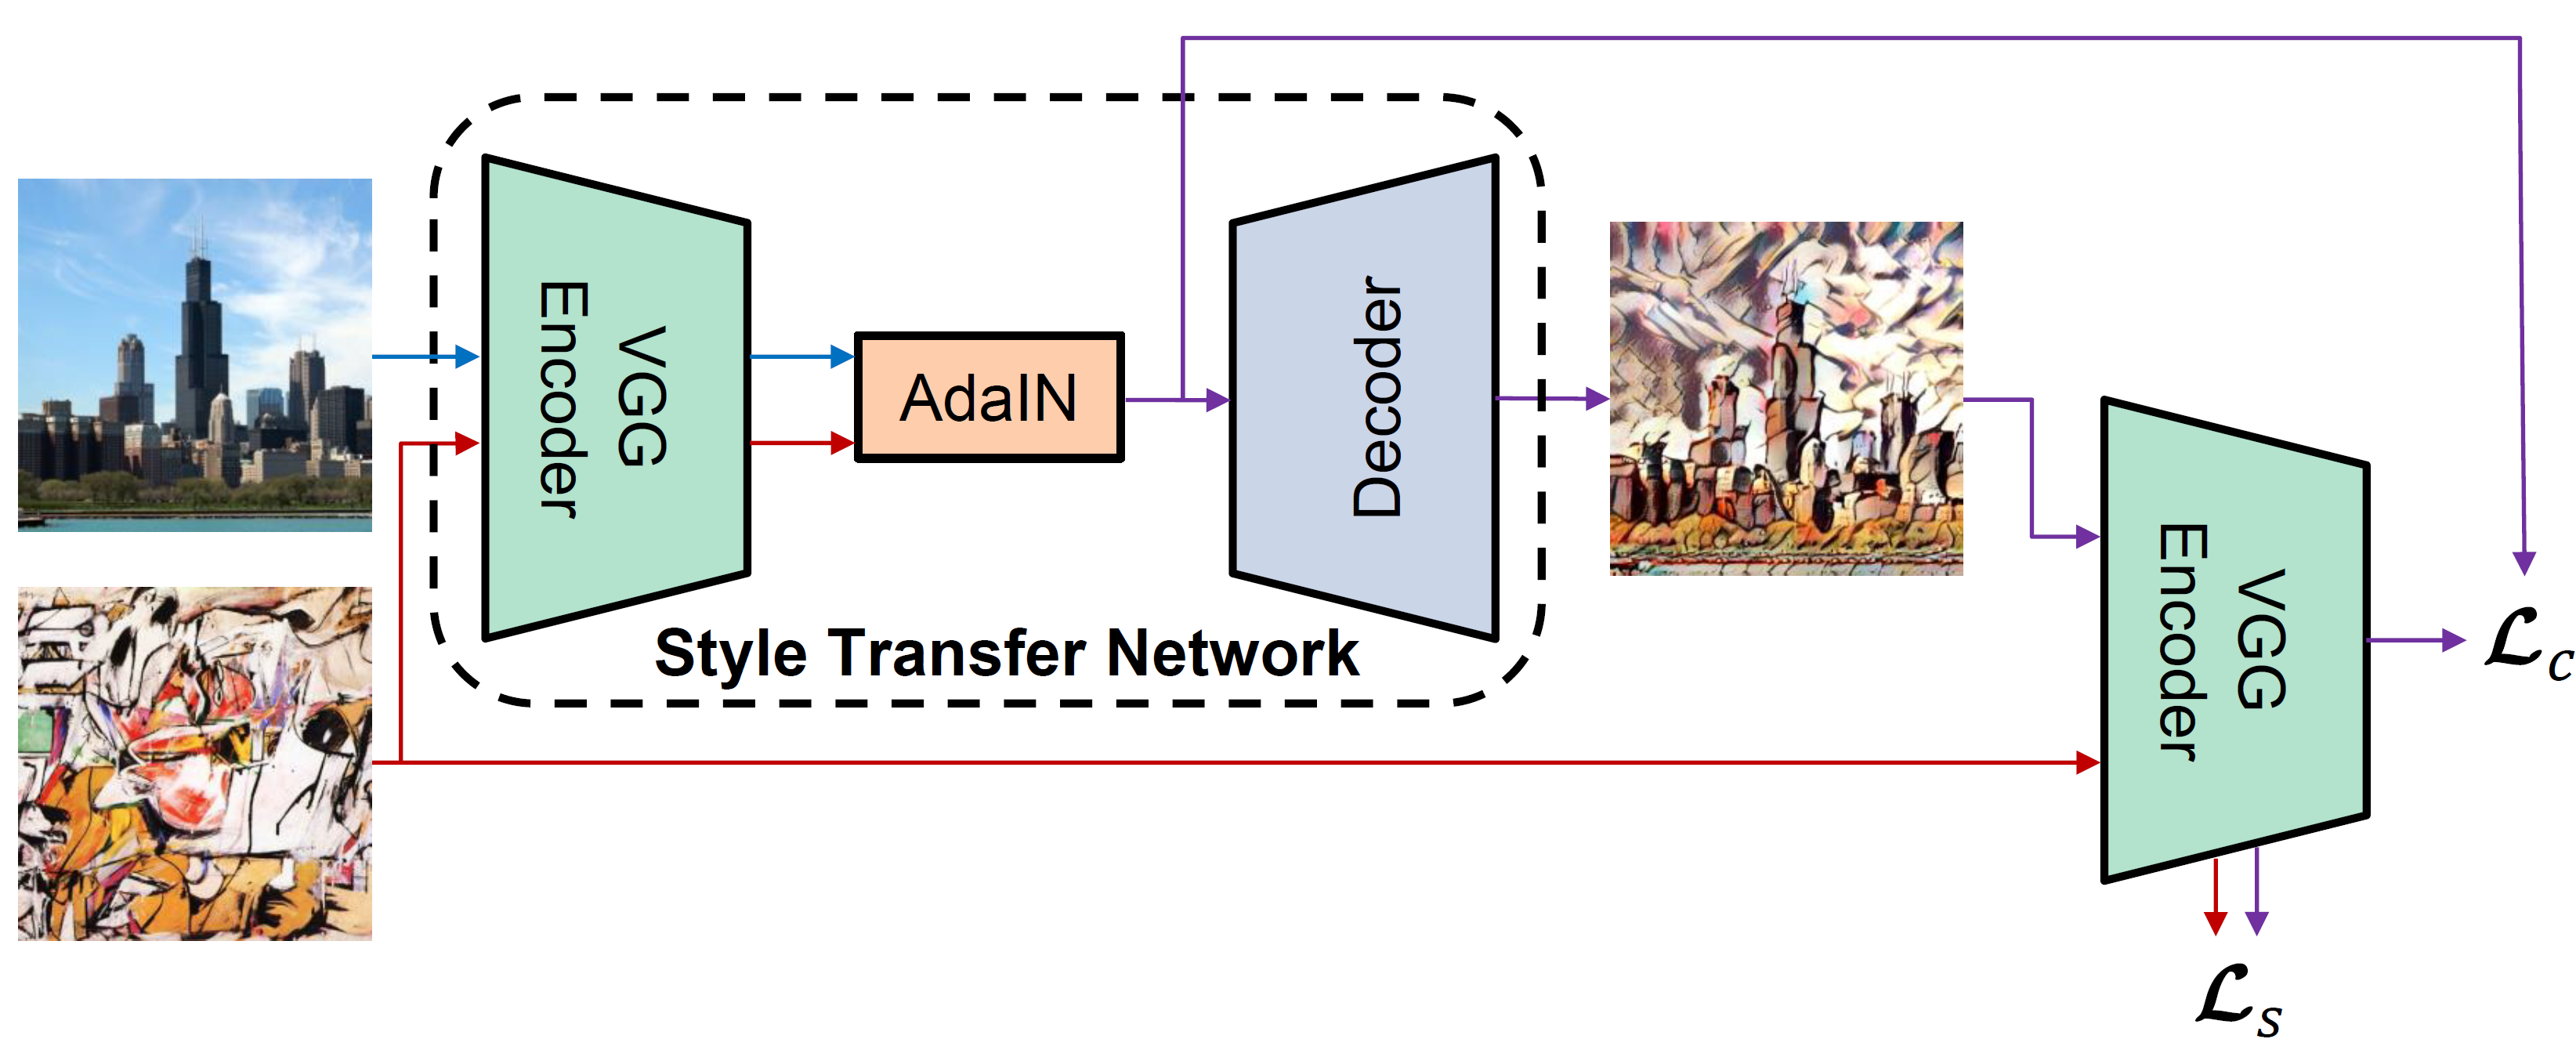
\includegraphics[width=0.48\textwidth]{adaptive_instance_normalization}
	}
\end{figure}

\subsubsection{Generative Adversarial Networks}
Among the first to use GAN are Isola et al. \cite{Isola2016}, who use cGAN.
However, their method still requires paired training samples.
Meanwhile, Taigman et al. \cite{Taigman2016} are doing research in unsupervised domain transfer.
Their network uses an autoencoder as the generator and they assume that the encoder is fixed between domains.
The discriminator has a ternary output and distinguishes between real, fake and reconstruction.
They add several new loss functions which check the consistency between the two domains (consistency loss) and whether $G$ performs perfect reconstruction (reconstruction loss).
For the encoder, they use a pre-trained network that is trained on paired samples though.
In order to make the network completely unsupervised, Yi et al.\cite{Yi2017} propose DualGAN, Kim et al. \cite{Kim2017} DiscoGAN and Zhu et al. \cite{Zhu2017b} CycleGAN, which are all three essentially the same proposal.
The entire model consists of two cycle-consistent networks where each translates from one domain to the other.
A cycle-consistent network will first translate the input to a target domain and then back to the original domain.
Each domain has a discriminator which compares the real input from one network with the fake from the other (adversarial loss).
In addition to this there's a cycle-consistency loss, which is the MSE between the input and the reconstructed image as you can see in Figure \ref{fig:style_transfer_algorithm_cyclegan}.
The goal is to minimize the adversarial and cycle-consistency loss, while maximizing the discriminators' accuracy.

\begin{figure}[h]
	\centering
	\captionbox{
		\label{fig:style_transfer_algorithm_cyclegan}
		The cycle-consistent network by Zhu et al. \cite{Zhu2017b}.
		Unsupervised image-to-image translation between domains $X$ and $Y$ is established by training the generators $G$, $F$ and discriminators $D_X$, $D_Y$.
		During training cycle-consistency loss is calculated under the assumption that $F(G(x))\overset{!}{=} x$ and $G(F(y))\overset{!}{=} y$.
	}{	
		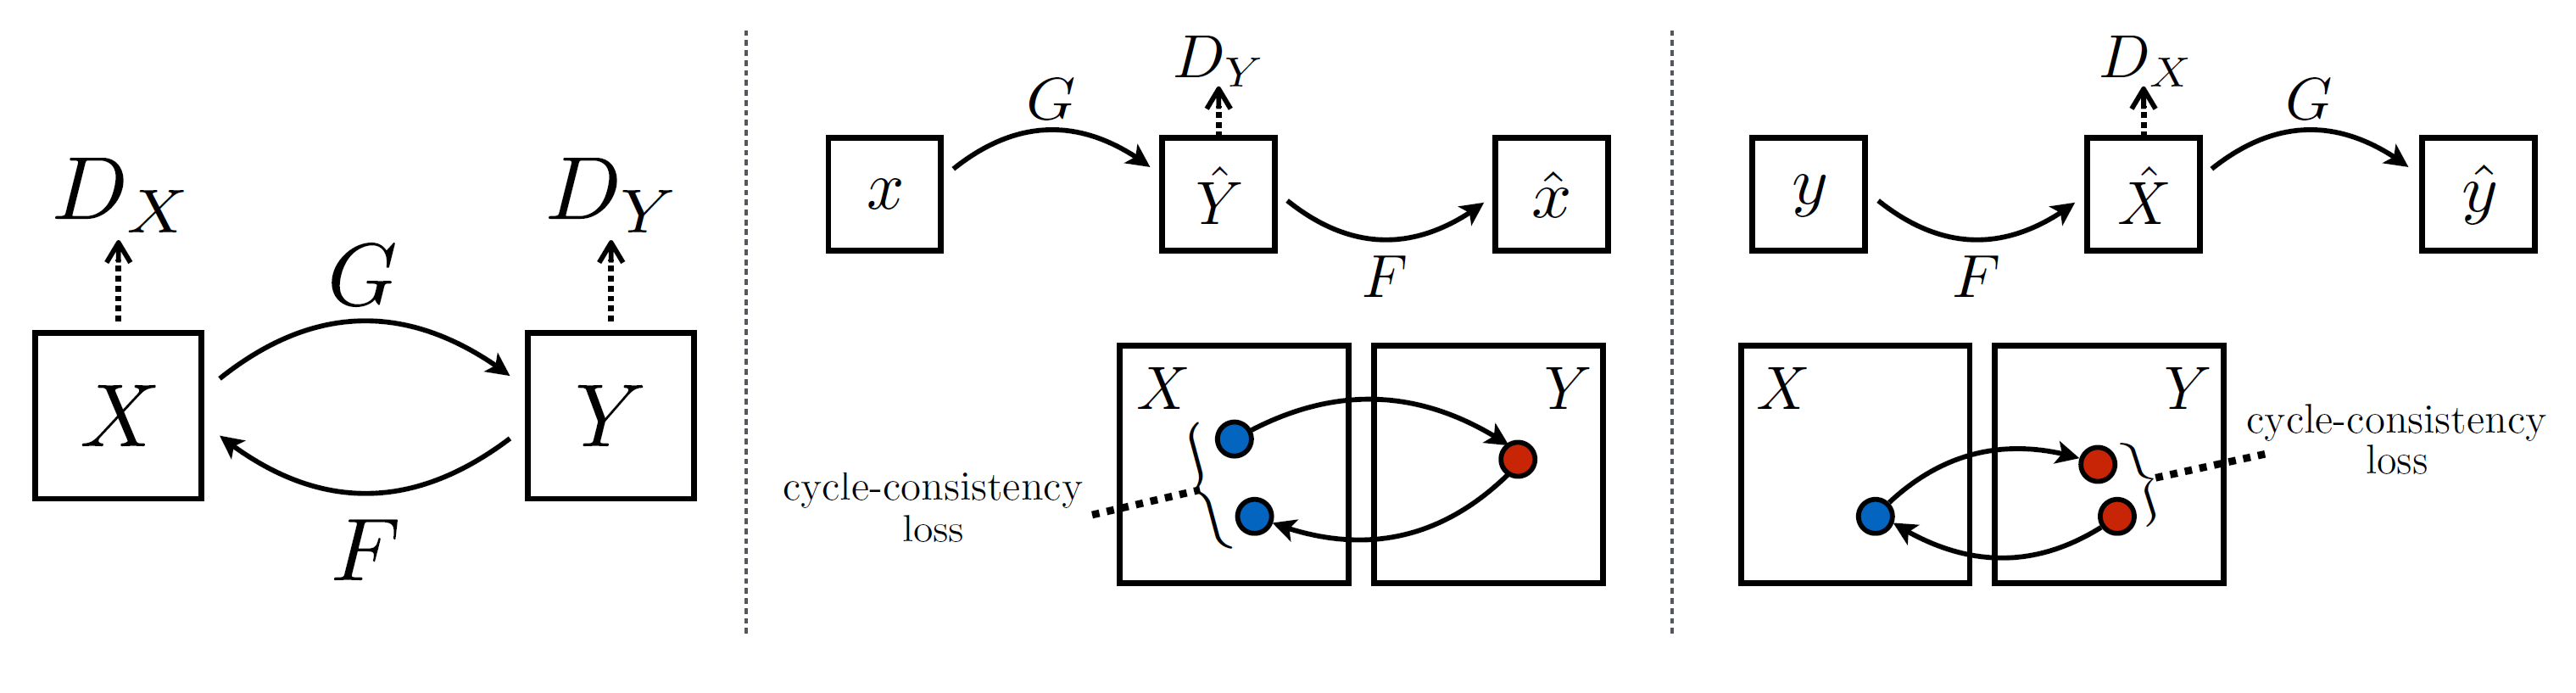
\includegraphics[width=0.48\textwidth]{style_transfer_algorithm_cyclegan}%
	}
\end{figure}

\subsection{Content-Based Image Retrieval}
Content-Based Image Retrieval (CBIR), a long-established research area, is the task of finding semantically matching or similar content images for a specified query image.
This has become increasingly relevant with the exponential growth of image and video data and the need to effectively search these image collections.
CBIR has been used specifically for person re-identification, remote sensing, medical image search, and shopping recommendations in online marketplaces, among many others \cite{Chen2021a}.
Image retrieval can be categorized into two different groups: Category Image Retrieval (CIR) and Instance Image Retrieval (IIR).
CIR's goal is to find images within the same category as the query, while IIR tries to find images with a particular instance given in the query image.
For IIR, Radenovic et al. \cite{Radenovic2017} train a VGG network from reconstructed 3D models obtained by retrieval and structure-from-motion methods.
This allows them to use the geometry and camera positions to enhance the feature extraction along with several other optimization techniques.
During training, they make use of the contrastive loss.
Contrastive loss is minimized when similar image pairs are close to each other in embedding space and different pairs are far away.

\subsection{Deep Learning in the Art domain}
Through digitization, analysis of art collections has become more efficient.
Artists are constantly inspiring and being inspired, and in order to correctly analyze the relation between paintings and artists, it's beneficial to have a method that finds their inspirations.
One way that can be achieved is by using image retrieval, which gives good results, but only when the works are visually similar.
In other cases, the inspiration is drawn from themes, which involve composition, lighting and poses.
Jenicek et al. \cite{Jenicek2019} propose finding these relations by analyzing the similarity between poses.
From a database of images the poses are estimated and normalized.
They then employ a two step process: With a query image and fast matching, they generate a shortlist of possible hits.
Afterwards, geometric validation filters out impossible alignments with the query image.
Their experiments show significant improvements over previous methods.
They also note some failure cases where pose estimation falls short, like failing to find keypoints or making associations with wrong poses.
To improve these shortcomings on Greek vases, Madhu et al. \cite{Madhu2020} apply style transfer to the COCO dataset with AdaIN in the style of those vases and use this for fine-tuning.
They use a top-down architecture with Faster R-CNN as detector and HRNet for pose estimation.
They also created their own small dataset to evaluate their improvements (Figure \ref{fig:related_papers_madhu}).
Kadish et al. \cite{Kadish2021} have the same idea and also use AdaIN to stylize the COCO dataset.
They randomly sample artworks from the Painter by Numbers dataset from Kaggle \cite{PainterByNumbers} for the style images and using it to fine-tune the Faster R-CNN network for object detection.
Both papers found an improvement in the performance of the networks on art collections.

\begin{figure}[h]
	\centering
	\captionbox{
		\label{fig:related_papers_madhu}
		Improvements to the state-of-the-art by Madhu et al. \cite{Madhu2020}.
	}{	
		\subcaptionbox{Original}[0.14\textwidth]{%
			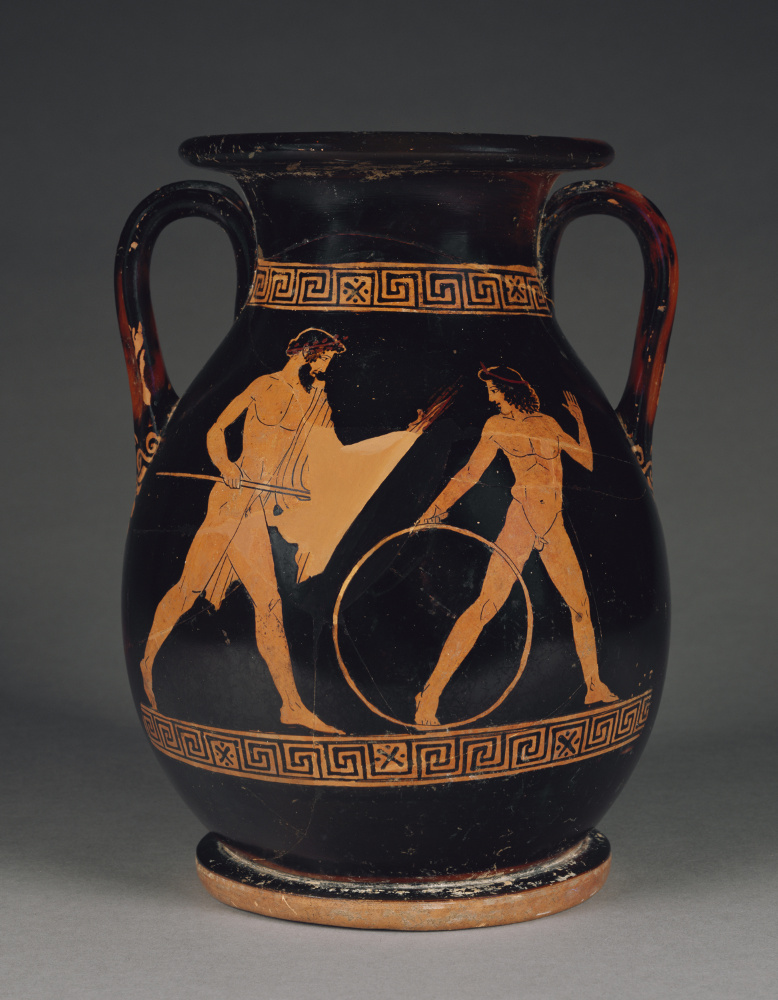
\includegraphics[width=0.14\textwidth]{related_papers_vase}%
		}
		\subcaptionbox{OpenPose}[0.14\textwidth]{%
			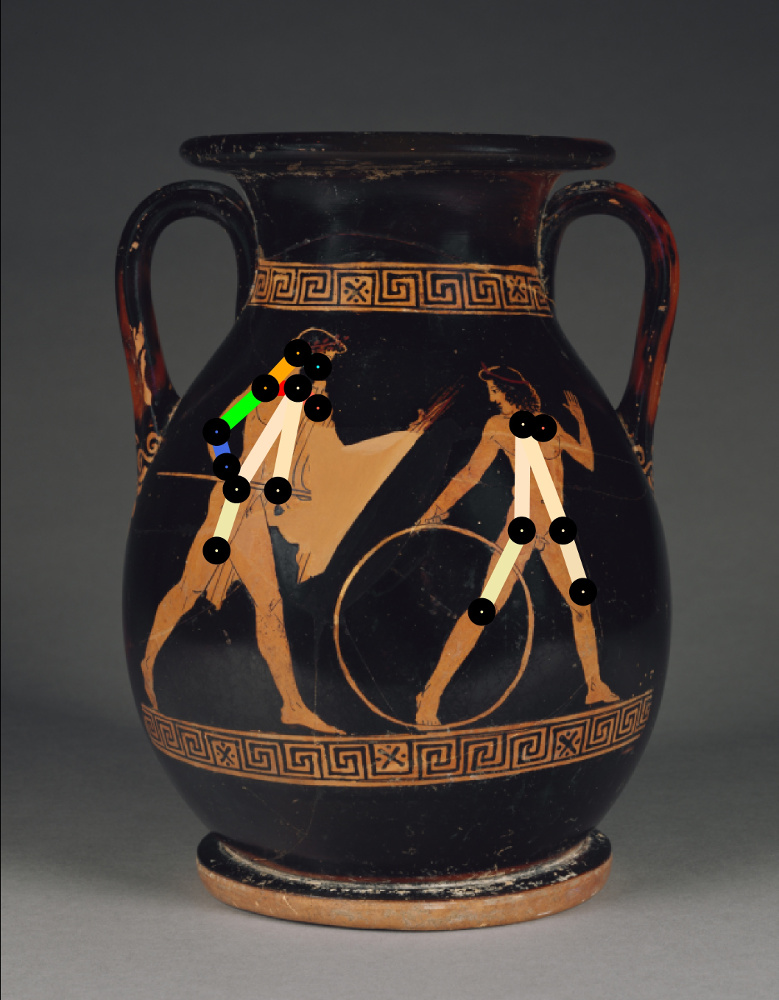
\includegraphics[width=0.14\textwidth]{related_papers_vase_sota}%
		}
		\subcaptionbox{Madhu et al.}[0.14\textwidth]{%
			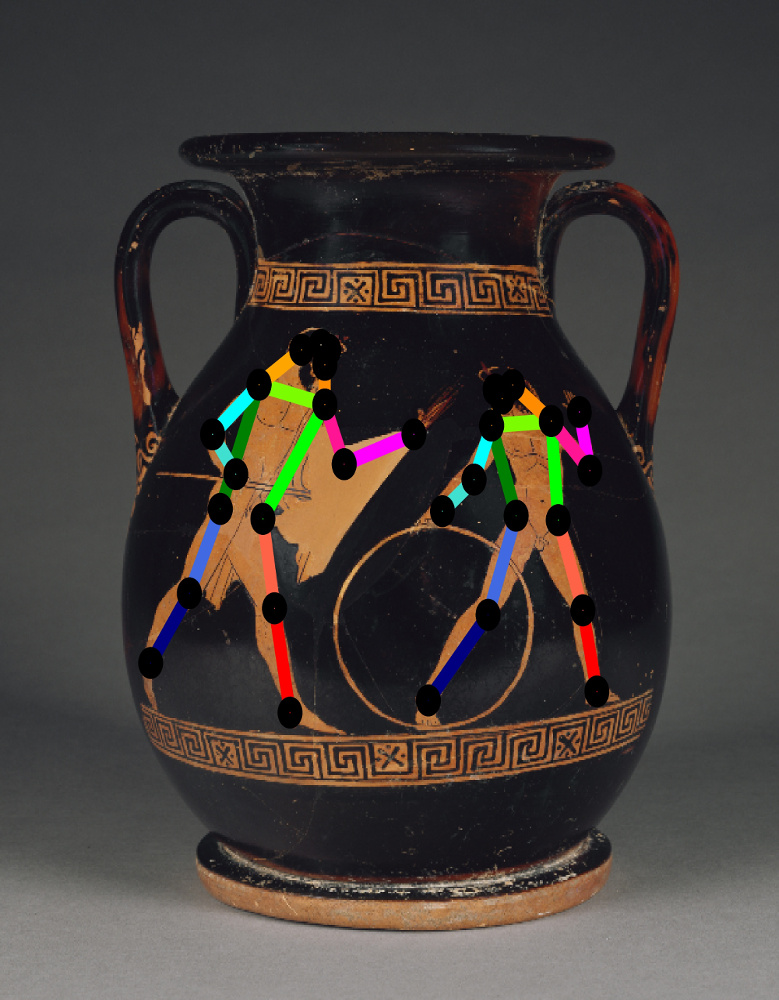
\includegraphics[width=0.14\textwidth]{related_papers_vase_stl}%
		}
	}
\end{figure}

\section{Datasets}
\subsection{Human Pose Estimation}
\subsubsection{Common Object in Context (COCO) Dataset \cite{Lin2014}}
COCO is a large-scale dataset for a wide range of computer vision algorithms.
For HPE, the set contains more than 200,000 images in which 250,000 persons are annotated.
Each person has 17 keypoints, a bounding-box and visibility labels.
This dataset has become the most popular for benchmarking.

\subsubsection{Human-Art Dataset \cite{Ju2023}}
Human-Art dataset bridges the gap between natural and artificial images.
The set contains 50,000 high-quality images with 123,000 annotated humans.
Each person has 17 keypoints, bounding boxes, self-contact points, and text information.

\subsection{Image Style Transfer}
\subsubsection{Arbitrary Style Transfer Image Quality Assessment Database (AST-IQAD) \cite{Chen2023}}
AST-IQAD is a set specifically made to measure style transfer.
It constructs the set around several inter-subjective characteristics and categories.
This means that these criteria of subjective evaluation are mostly agreed upon across a group of people.
Among those are: color tone, brush stroke, distribution of objects, and contents.
It also declares a set of style images.

\subsubsection{WikiArt Dataset \cite{Saleh2015}}
WikiArt consists of 80,000 fine-art paintings.
All are annotated for 27 styles, 60,000 are annotated for 20 genres and 20,000 for 23 artists.

\section{Methodology}
The goal is to improve pose estimation on art collections.
SWAHR and ViTPose will be fine-tuned on an COCO dataset which is augmented with synthetic COCO images.
This needs a style transfer model that is trained to do a transformation between an art movement and realistic images.
For this, AdaIN and CycleGAN will be analyzed.
The style transfer models will be trained on three datasets of different art movements.

\subsection{Style Transfer}
\subsubsection{Datasets}
None of the selected models has any pre-trained weights for certain art movements, so new models need to be made.
The WikiArt dataset will be used to assemble different datasets and specifically on the Baroque, Renaissance and Impressionism styles.
The impressionist style is chosen because it is more colorful and abstract than the others.
Baroque and Renaissance are both very dark and very similar in style, but renaissance artworks are just a bit more stylized.
For each art movement, a subset needs to be created with images that contain full body poses as well as crowded images, as this is what the pose estimation models are trained on.
While there's a high variation of genres in the WikiArt dataset, they do not adequately subdivide the dataset for this problem.
It is important then to have a consistent style in each dataset which is not possible by just splitting the genres provided by WikiArt.
To achieve this, the Content Based Image Retrieval (CBIR) model by Radenovic et al. \cite{Radenovic2017} is used.
Using a query image it can find similar looking images.
This results in four datasets: The photograph dataset which consists of 825 images, the baroque dataset with 518 images, the impressionism dataset with 780 images and the renaissance dataset consisting of 790 images.
Figure \ref{fig:style_transfer_dataset} shows the kind of images that can be found in the datasets where the human figure is central.

\begin{figure}[h]
	\centering
	{
		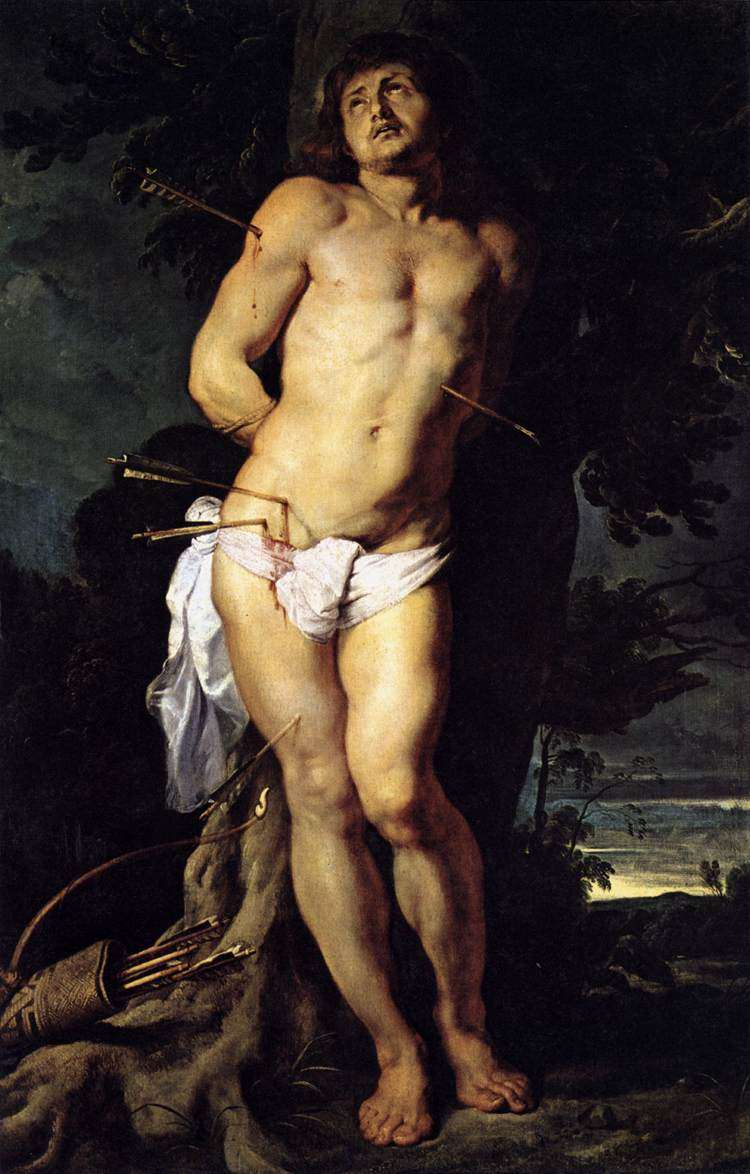
\includegraphics[height=0.9in]{15_96_peter-paul-rubens_st-sebastian}
		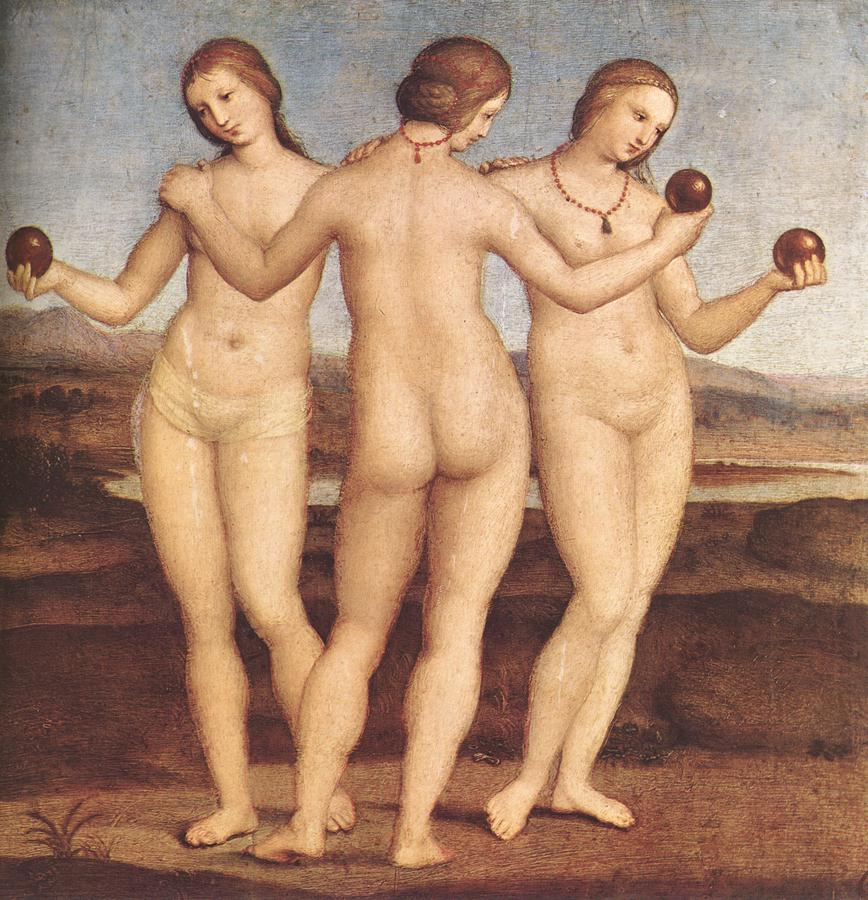
\includegraphics[height=0.9in]{26_4_raphael_the-three-graces-1505}
		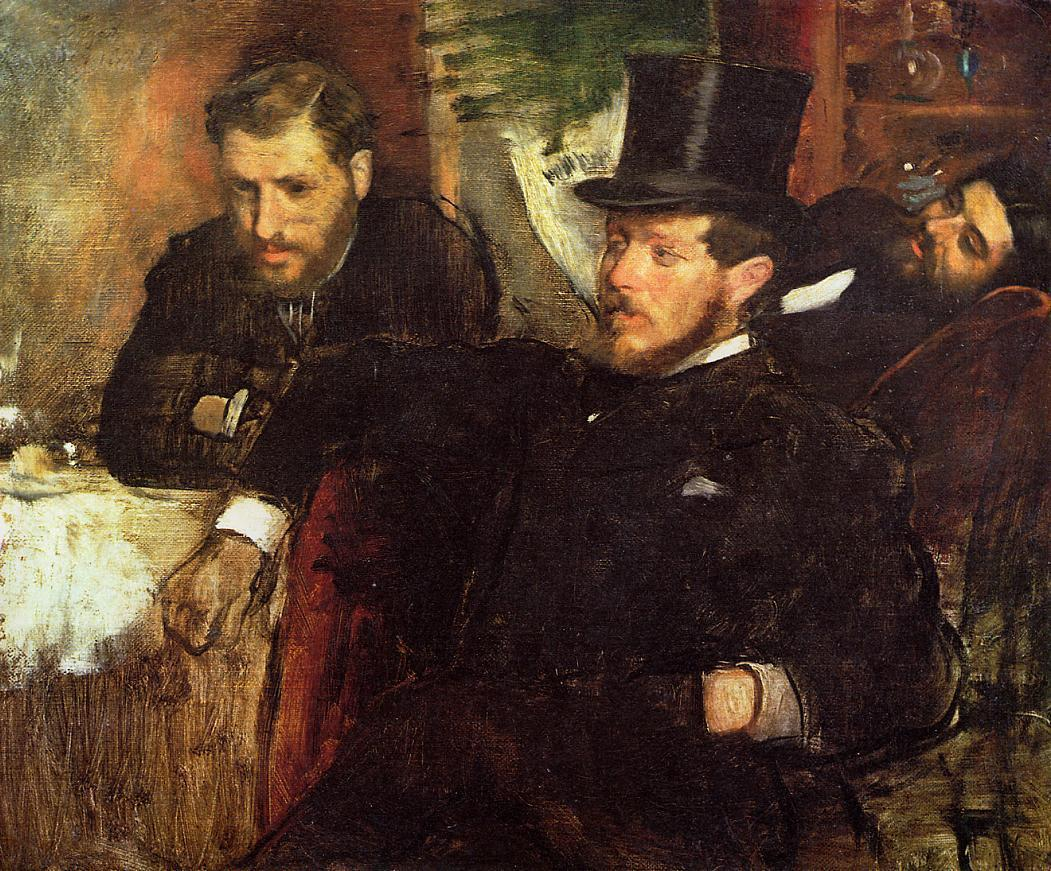
\includegraphics[height=0.9in]{37_79_edgar-degas_jeantaud-linet-and-laine-1871}
		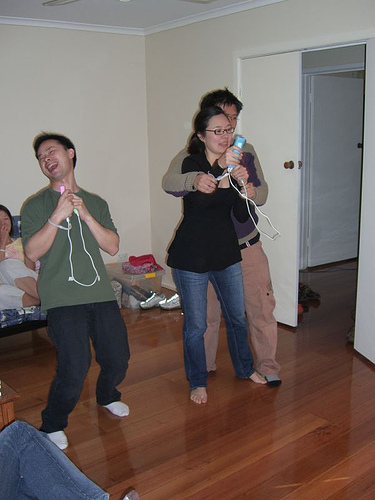
\includegraphics[height=0.9in]{22_21_000000084015 - kopie}\\
		\vspace{0.05in}
	}
	{
		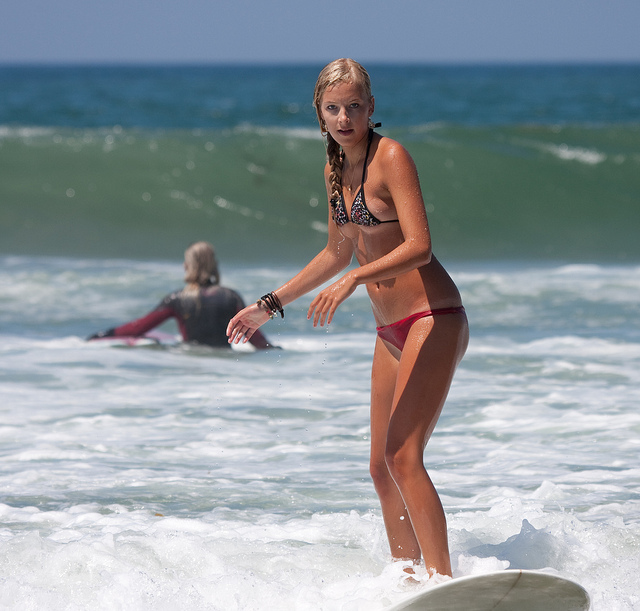
\includegraphics[height=0.9in]{28_1_000000032850}
		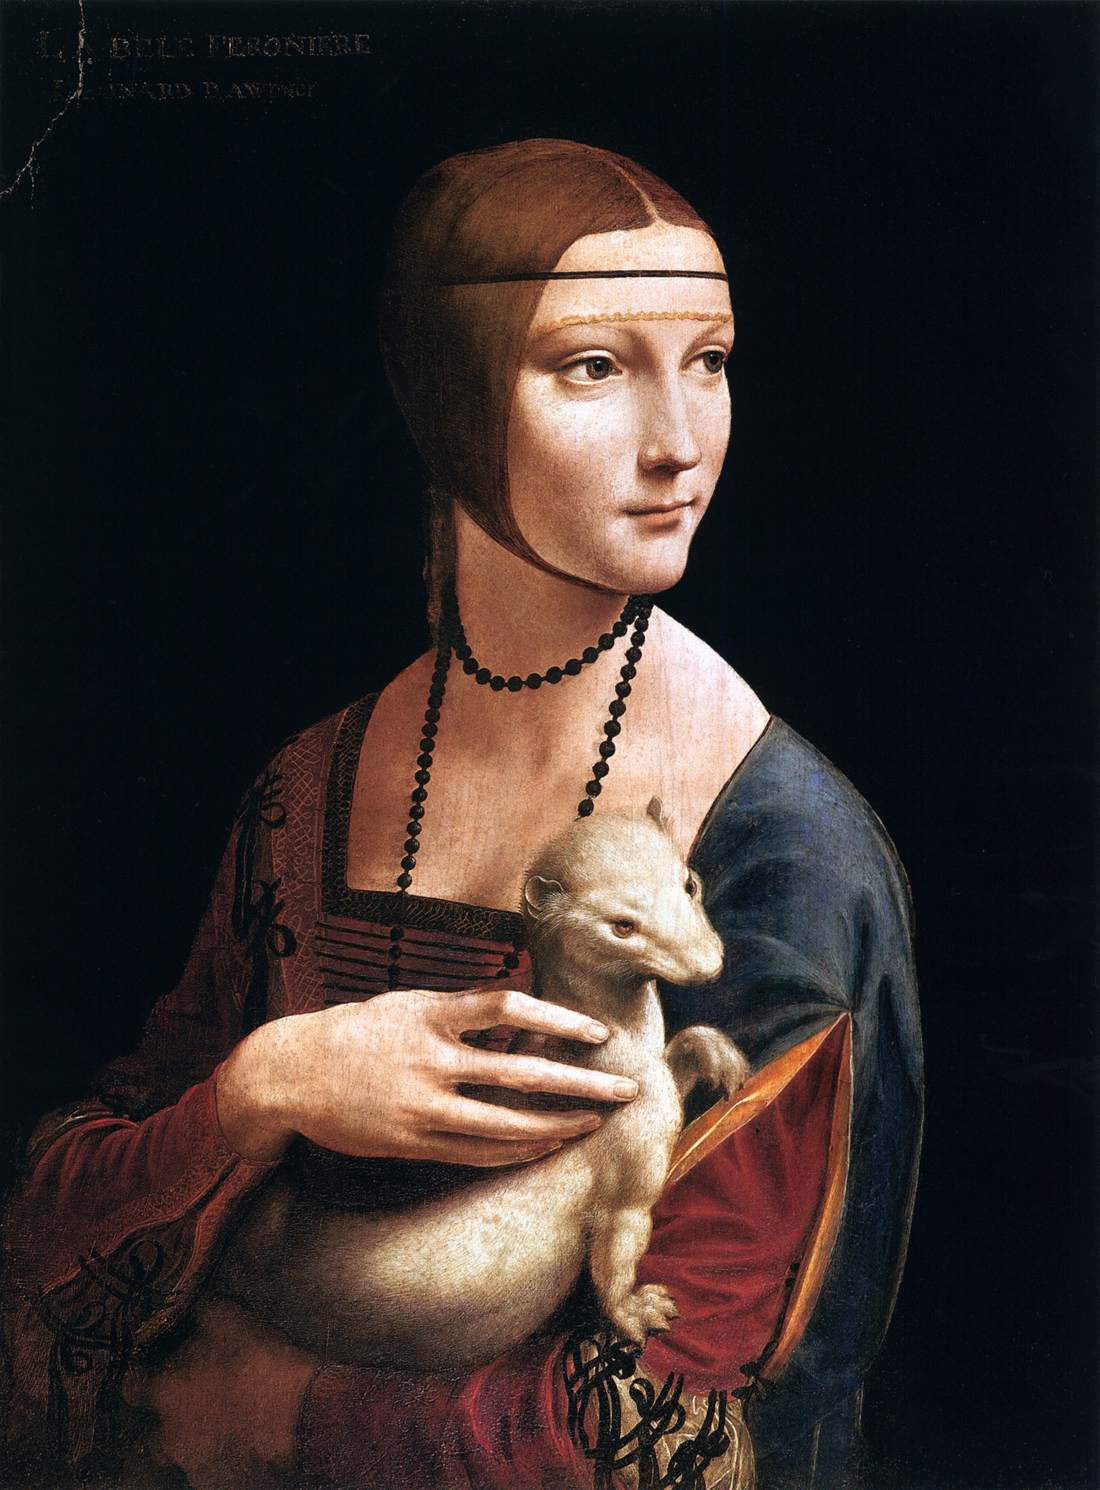
\includegraphics[height=0.9in]{16_10_leonardo-da-vinci_the-lady-with-the-ermine-cecilia-gallerani-1496}
		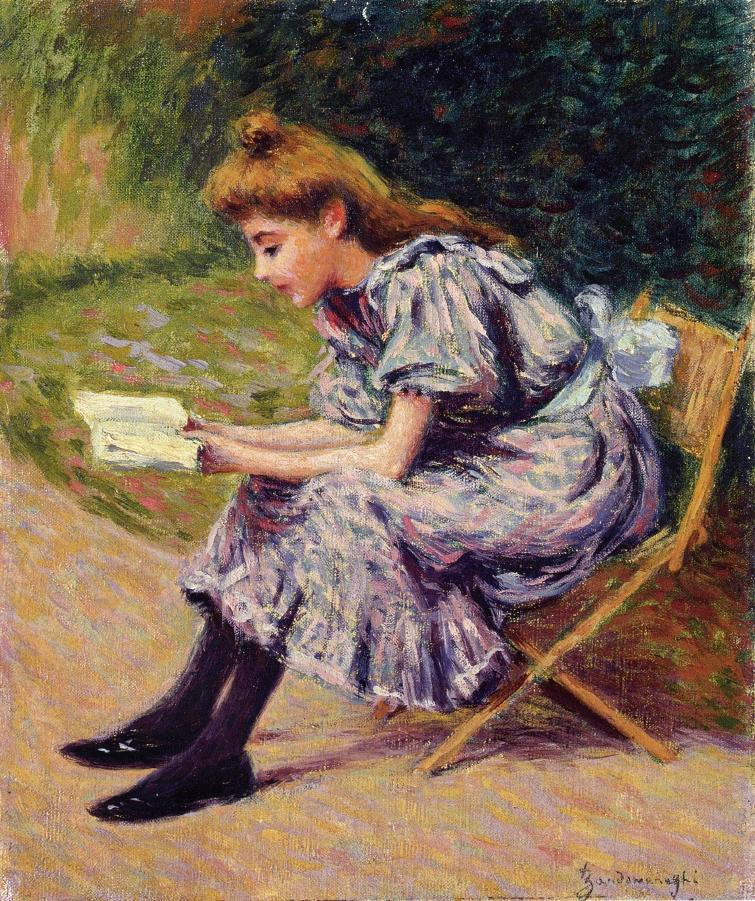
\includegraphics[height=0.9in]{36_65_federico-zandomeneghi_the-reader}
		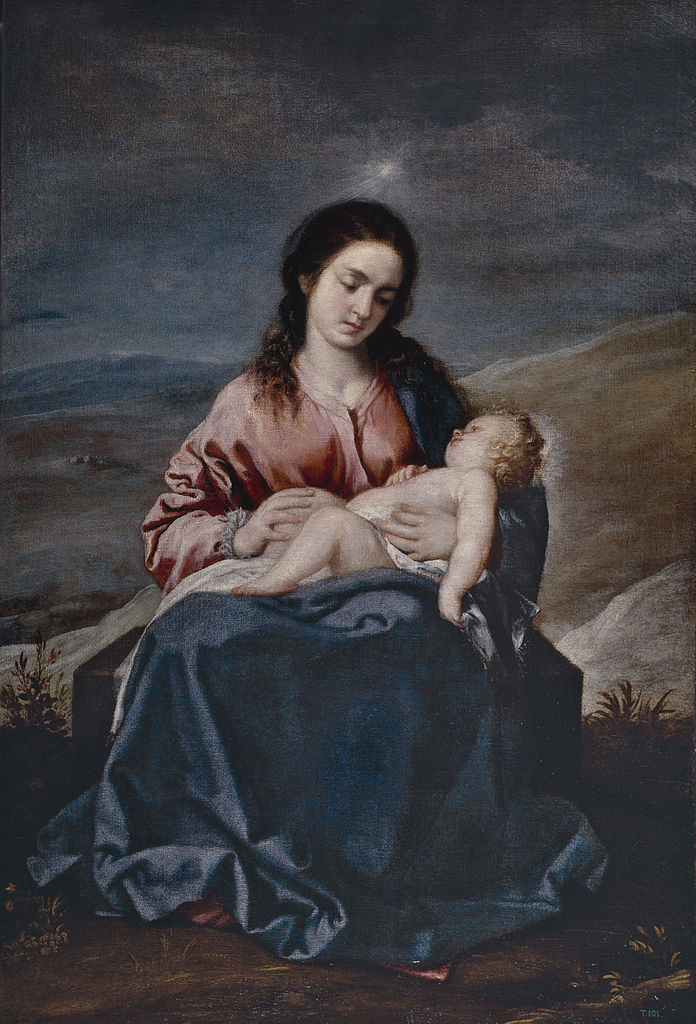
\includegraphics[height=0.9in]{24_10_alonzo-cano_the-virgin-and-child-1643}
	}
	\caption{A selection from the different datasets. The human figure is central to all images.}
	\label{fig:style_transfer_dataset}
\end{figure}

\subsubsection{Training}
From the selected models only CycleGAN requires training.
AdaIN can use any arbitrary style from a content image to do style transfer.
This eliminates the need to train a new model for it and the pre-trained model can be used for the experiments.
CycleGAN will be trained with the provided default parameters.
No hyperparameter tuning will be done as the goal is to measure the performance between different approaches and not optimize a single model.

\begin{figure*}[t]
	\centering
	\subcaptionbox{Content}{
        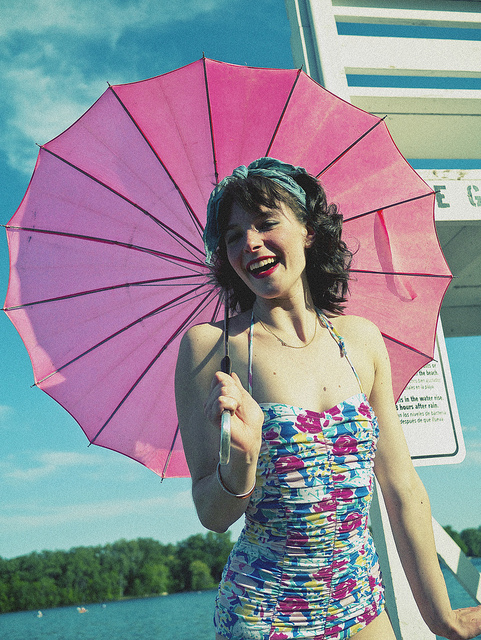
\includegraphics[width=0.11\textwidth]{000000000036}
	}
	\subcaptionbox{CycleGAN. Left to right: Baroque, Impressionism and Renaissance}{
        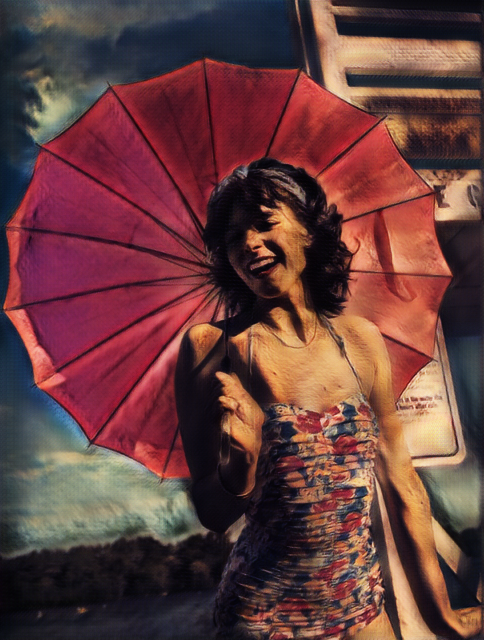
\includegraphics[width=0.11\textwidth]{000000000036_baroque_200}
        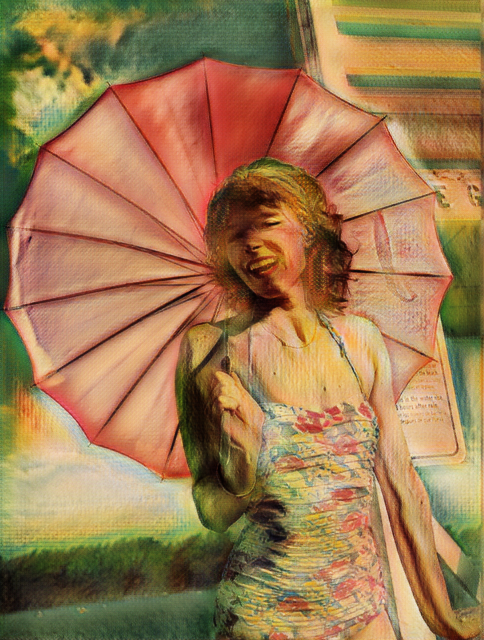
\includegraphics[width=0.11\textwidth]{000000000036_impressionism_2}
        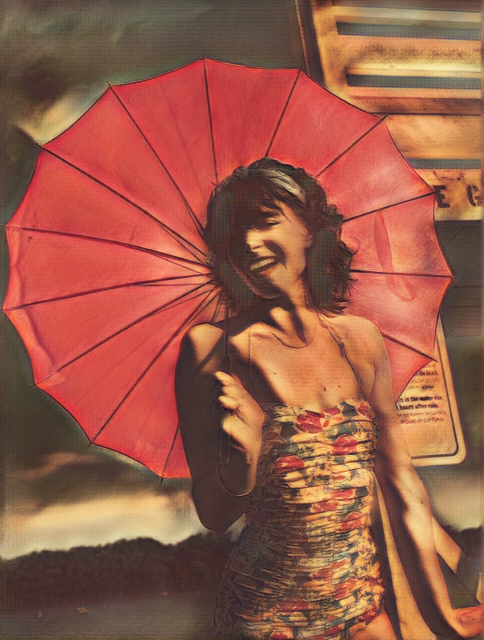
\includegraphics[width=0.11\textwidth]{000000000036_renaissance_2}
	}
	\subcaptionbox{AdaIN. Paired with style image from left to right: Baroque, Impressionism and Renaissance. } {
		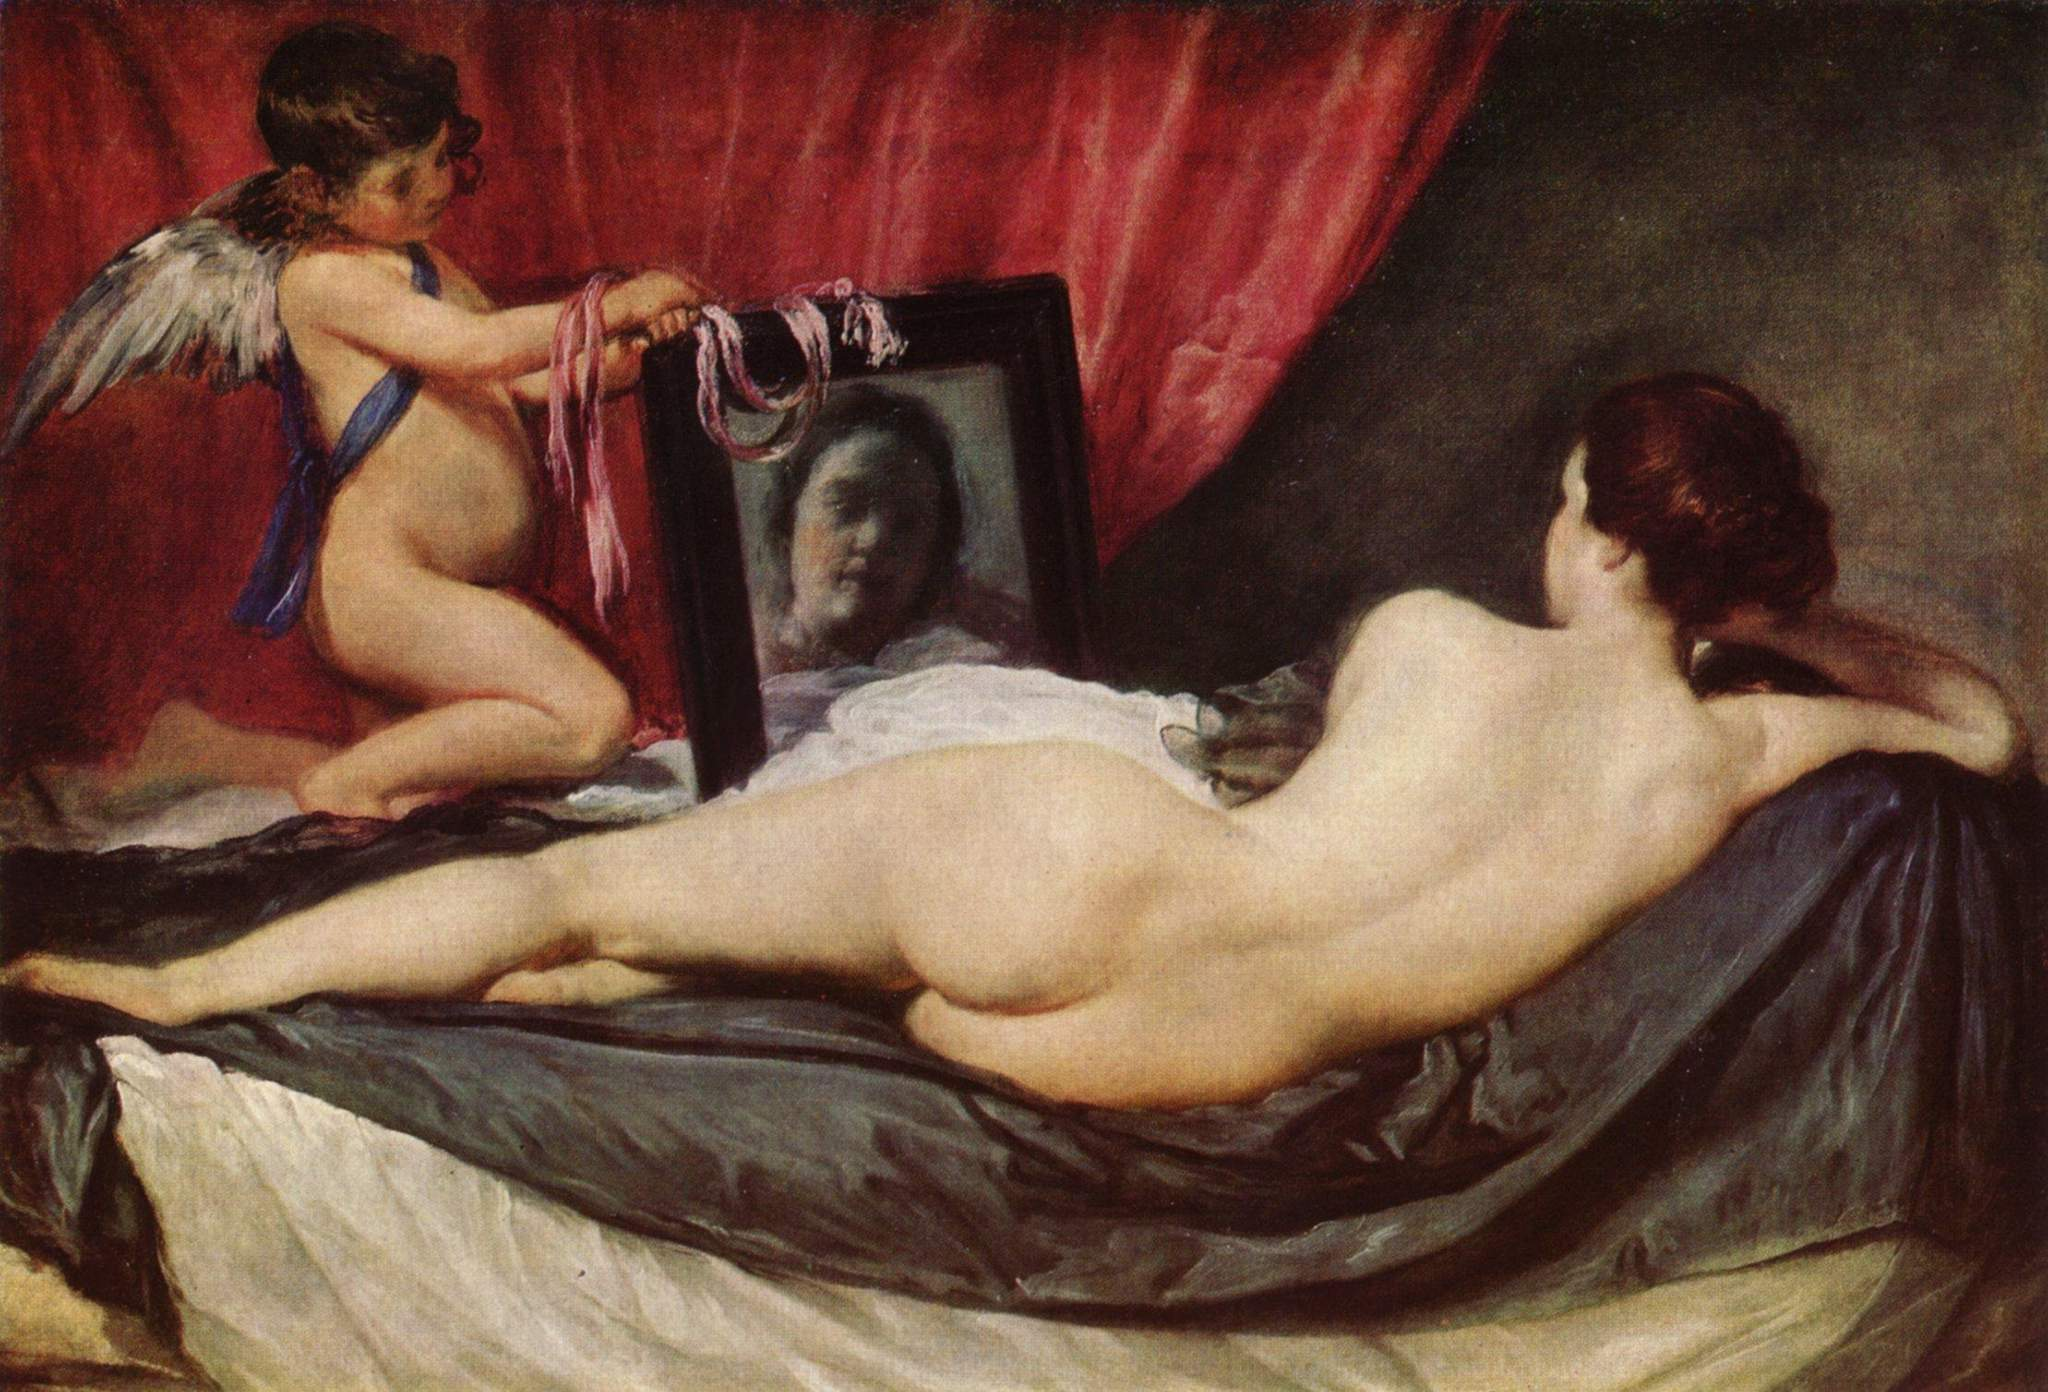
\includegraphics[height=1in]{22_22_diego-velazquez_the-rokeby-venus-1648}
		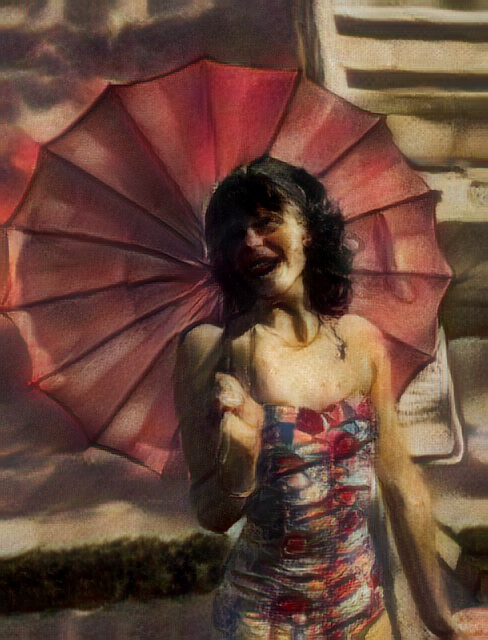
\includegraphics[height=1in]{000000000036_adain_baroque_a}
        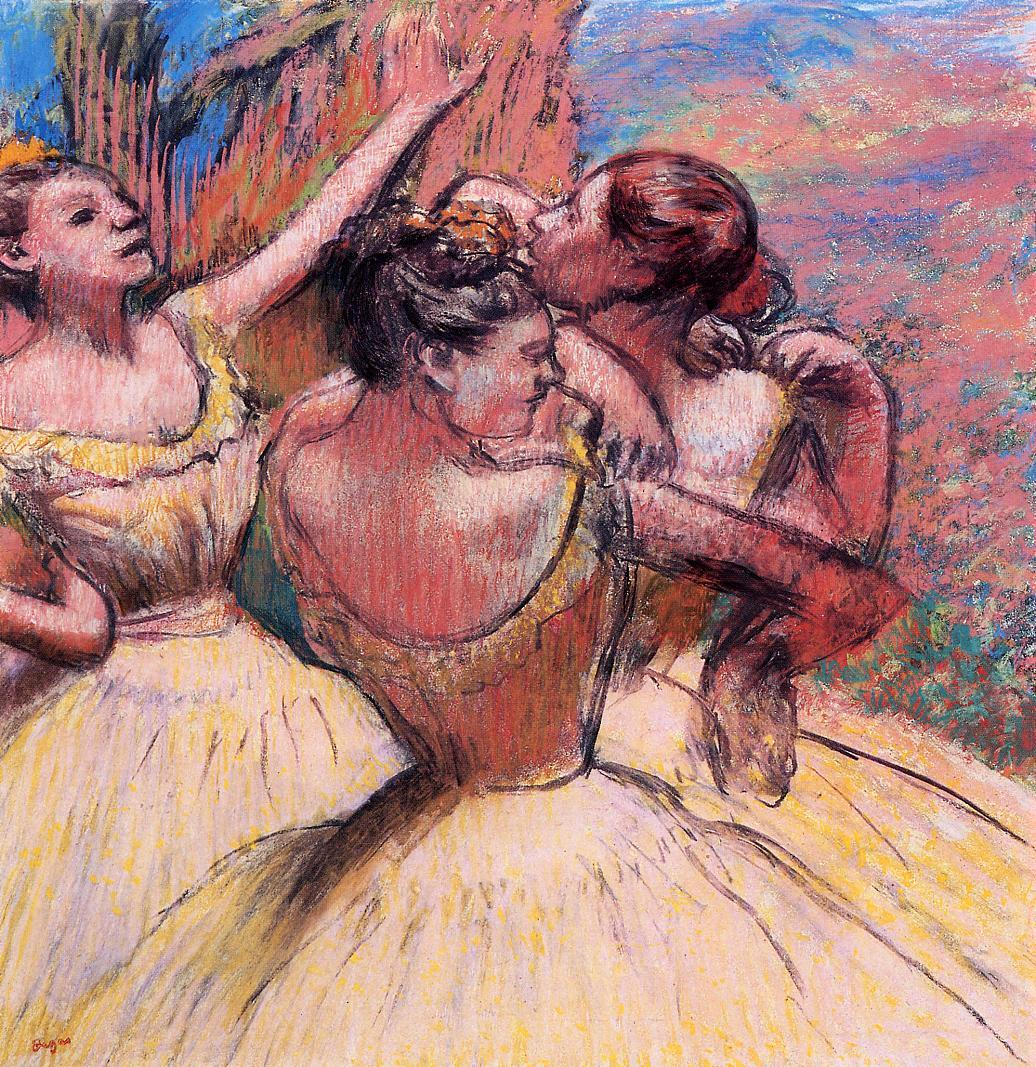
\includegraphics[height=1in]{22_91_edgar-degas_three-dancers}
        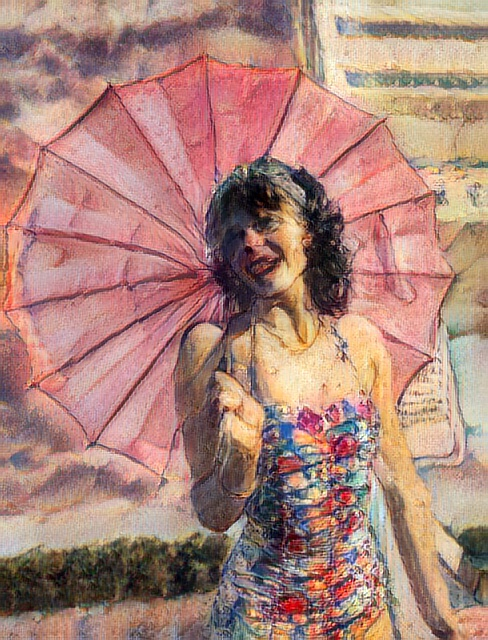
\includegraphics[height=1in]{000000000036_adain_impressionism_a}
        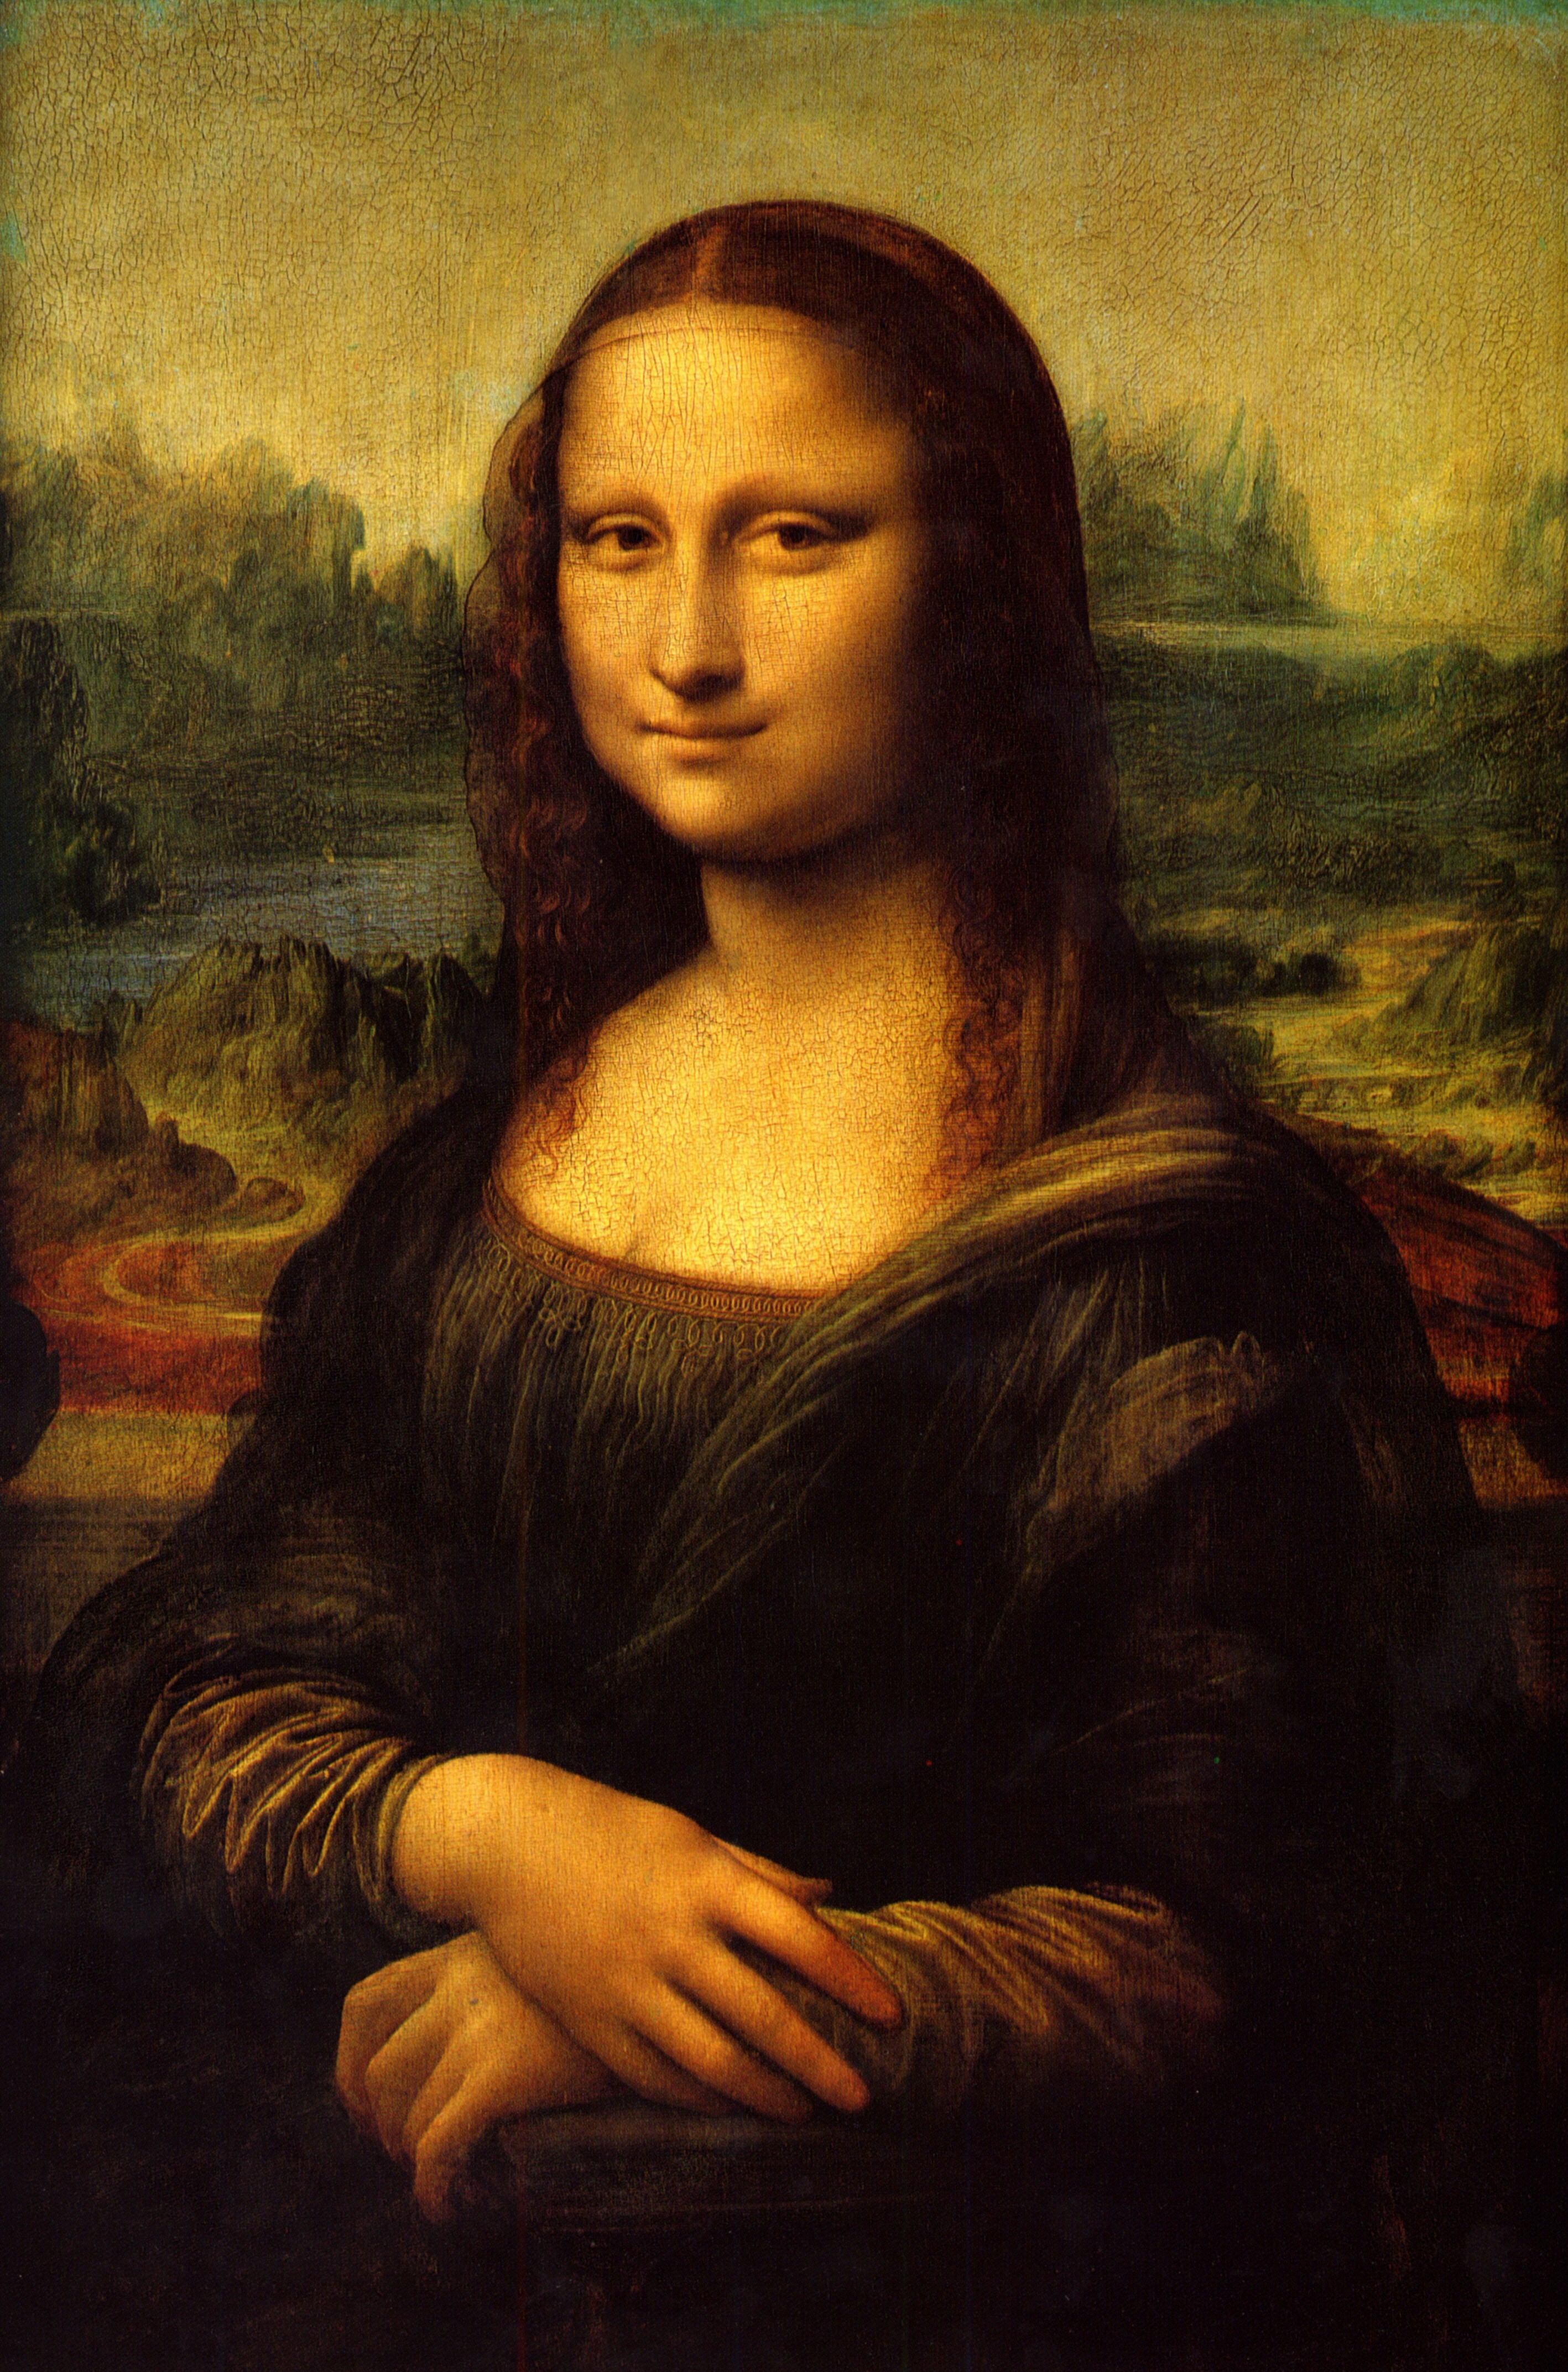
\includegraphics[height=1in]{15_11_leonardo-da-vinci_mona-lisa}
        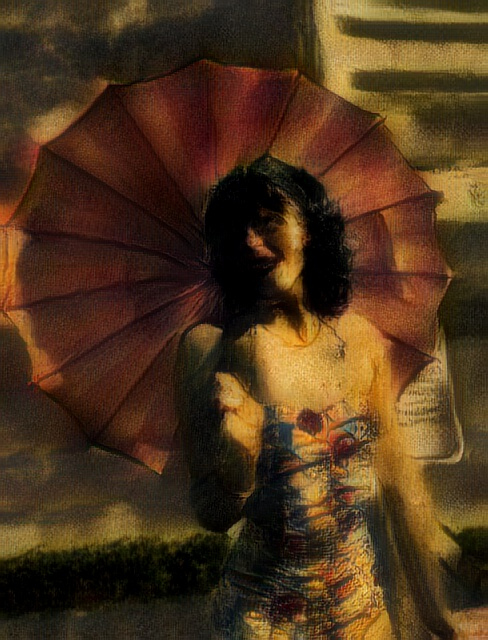
\includegraphics[height=1in]{000000000036_adain_renaissance_b}
    }
	\caption{AdaIN abstracts the features more than CycleGAN, while StarGAN experiences modal collapse.}
	\label{fig:difference_AdaIN_CycleGAN}
\end{figure*}

\subsubsection{Qualitative Evaluation}
As shown in Figure \ref{fig:difference_AdaIN_CycleGAN}, AdaIN removes more of the details of the content than CycleGAN does, but as expected the style transfer is completely dependent on the style image used.
CycleGAN does look like it is able to capture the general style of the learned art movements, e.g. baroque and renaissance are dark, and impressionism is colorful.
All in all, the results are very disappointing as none of the images look like they're a painting from a different time.

\subsubsection{Quantitative Evaluation}
To evaluate the trained models, Perceptual Distance (PD), Fréchet Inception Distance (FID), Inception Score (IS) and Learned Perceptual Image Patch Similarity (LPIPS) are used.
Before applying the evaluation metrics there needs to be an adequate dataset to do meaningful measurements on first.
Two datasets are considered for this purpose, AST-IQAD, but since it works with different kinds of content, and the content of the problem only focuses around persons, a custom dataset is created that focuses around persons.
This is created the same way the style transfer datasets were created.
In Table \ref{tab:performance_style_transfer_by_dataset}, the results of the evaluation are available.
AdaIn performs better than CycleGAN, impressionism does the best out of all of the styles and the custom dataset has a slightly better evaluation.

\begin{table}[h]
    \setlength\tabcolsep{4pt}
    \vspace{0.2em}
    \caption{Performance comparison of Style Transfer measured by various metrics grouped by dataset; Perceptual Distance (PD), Inception score (IS), Fréchet Inception Distance (FID) and Learned Perceptual Image Patch Similarity (LPIPS).}
    \begin{center}
    \footnotesize
    \label{tab:performance_style_transfer_by_dataset}
    \begin{tabular}{ l|cccc }
        \hline
        \bf{Method}&\bf{PD}&\bf{IS}&\bf{FID}&\bf{LPIPS}\cr
        \hline
        \multicolumn{5}{c}{\bf{AST-IQAD Dataset}}\cr
        \multicolumn{5}{c}{\bf{Baroque}}\cr
        \hline
        AdaIN & \textbf{10.734} & \textbf{8.975} & \textbf{265.036} & 0.626 \cr
        CycleGAN & 14.670 & 10.850 & 272.652 & \textbf{0.633} \cr
        \hline 
        \multicolumn{5}{c}{\bf{Impressionism}}\cr
        \hline
        AdaIN & \textbf{10.671**} & \textbf{8.453} & \textbf{246.736} & 0.710 \cr
        CycleGAN & 14.160 & 10.046 & 247.468 & \textbf{0.721} \cr
        \hline 
        \multicolumn{5}{c}{\bf{Renaissance}}\cr
        \hline
        AdaIN & \textbf{10.671**} & \textbf{8.453} & \textbf{246.736} & 0.710 \cr
        CycleGAN & 14.160 & 10.046 & 247.468 & \textbf{0.721}\cr
        \hline 
        \multicolumn{5}{c}{\bf{Custom Dataset}}\cr
        \multicolumn{5}{c}{\bf{Baroque}}\cr
        \hline
        AdaIN & \textbf{10.507*} & \textbf{6.639**} & \textbf{195.487**} & \textbf{0.654**} \cr
        CycleGAN & 13.435 & 7.137 & 200.299 & 0.635 \cr
        \hline
        \multicolumn{5}{c}{\bf{Impressionism}}\cr
        \hline
        AdaIN & 13.435 & \textbf{4.974*} & \textbf{177.581*} &\textbf{0.737*} \cr
        CycleGAN & \textbf{12.456} & 6.047 & 190.658 & 0.711 \cr
        \hline
        \multicolumn{5}{c}{\bf{Renaissance}}\cr
        \hline
        AdaIN & \textbf{11.472} & \textbf{5.156**} & \textbf{197.560**} & \textbf{0.693} \cr
        CycleGAN & 12.962 & 7.825 & 200.920 & 0.678 \cr
        \hline
    \end{tabular}
    \end{center}
    \leavevmode
    \footnotesize
    * the best result overall. \\
    ** the best result for the style.
\end{table}

\section{Experiments}
To improve pose estimation, SWAHR and ViTPose will be trained on several different stylized datasets.
A combination of the COCO dataset and the stylized dataset is used, and one with only the stylized dataset.
The stylized datasets are created by applying both CycleGAN and AdaIN to the COCO dataset.
One with a mixture of the baroque, impressionism and renaissance models, and one with only the impressionism model.
This results in a combination of 16 models.
The experiments will be conducted on the COCO-dataset as well as the Human-Art dataset.
While the problem specifically tries to improve the performance on artworks, it's still interesting to also validate the results on the COCO-dataset.

\subsubsection{Styled COCO Datasets}
Since AdaIN requires a style image, the images used for training the CycleGAN models were used for this purpose.
The style dataset was cycled through to transform the COCO dataset with AdaIN.
The decision to not use one image as a representation for each style was made so that the dataset is more generalized.
Afterwards, a dataset was created from a mixture of baroque, impressionism and renaissance stylized images, and one of only the impressionism style.
For each, a version was made which is appended to the COCO dataset and one that stands on its own.

\subsubsection{Training}
All models are trained with the default parameters initiating the weights with the pre-trained model.
They're trained for 200 epochs.
As a control, 2 models are trained without initiating weights these were trained for the default 300 epochs.

\subsubsection{Results}
For the SWAHR network, shown in table \ref{tab:experiments_style_transfered_pose_estimation_coco}, the best results are found with the model trained on the COCO + AdaIN mixed style transfer dataset.
The second best network was trained on the COCO + CycleGAN mixed style transfer dataset.
For the ViTPose network, the best results are with COCO + CycleGAN mixed and COCO + CycleGAN impressionism being the second best.
For AdaIN, there's a falloff of 7 to 10\% AP between the datasets with COCO and the ones without.
For CycleGAN, this falloff is less; between 0.2 and 4\% AP.
The best precision is found using the SWAHR model, while ViTPose has the honor of having the best recall.
Table \ref{tab:difference_style_transfered_pose_estimation_coco} compares the best models with the baseline.
It shows that the pre-trained SWAHR model has the best precision of all of the models and trained on the COCO + AdaIN Mixed style transfer dataset, SWAHR also has the second best precision.
ViTPose trained on COCO + CycleGAN mixed style transfer dataset has the best recall.
The networks trained from the ground up don't have any significant difference between the other networks.

The results on the Human-Art dataset are shown in table \ref{tab:experiments_style_transfered_pose_estimation_humanart}.
Here, one dataset takes the crown.
Both SWAHR as well as ViTPose have the best results for the models trained on the COCO + CycleGAN mixed style transfer dataset.
The second best model for SWAHR is trained on the COCO + AdaIN mixed dataset and for ViTPose this is the one trained on COCO + CycleGAN impressionism.
The falloff between the COCO and non-COCO datasets is between 5 to 9\% AP for AdaIN, and 2 to 3\% AP for CycleGAN.
The best precision and recall belongs to the SWAHR models.
Comparing the best models to the baseline (Table \ref{tab:difference_style_transfered_pose_estimation_humanart}), they still remain the best models overall with an increase of 3 to 5\% AP.
There's no significant difference between the non-initialized and bootstrapped networks.

\begin{table}
    \setlength\tabcolsep{4pt}
    \caption{Comparing the best models from the experiments on the COCO dataset with the baseline metrics. }
    \begin{center}
    \footnotesize
    \label{tab:difference_style_transfered_pose_estimation_coco}
    \begin{tabular}{ l|ccccc|ccccc }
        \hline
        \bf{Method}&\bf{AP}&\bf{AP$^{50}$}&\bf{AR}&\bf{AR$^{50}$}\cr
        \hline
        Pre-trained SWAHR & \bf{0.687*} & \bf{0.881*} & 0.737 & 0.904 \cr
        Pre-trained ViTPose & 0.588 & 0.832 & 0.723 & 0.906 \cr
        SWAHR & 0.620 & 0.830 & 0.710 & 0.891 \cr
        ViTPose & 0.609 & 0.847 & 0.740 & 0.918 \cr
        SWAHR COCO + AdaIN Mixed & \bf{0.679**} & \bf{0.874**} & 0.732 & 0.902 \cr
        ViTPose COCO + CycleGAN Mixed & 0.635 & 0.861 & \bf{0.763*} & \bf{0.925*} \cr
        \hline
    \end{tabular}
    \end{center}
    \leavevmode
    \footnotesize
    * the best result overall.\\
    ** the best result without pre-trained models.
\end{table}

\begin{table}
    \setlength\tabcolsep{4pt}
    \caption{Comparing the best models from the experiments on the Human-Art dataset with the baseline metrics. }
    \begin{center}
    \footnotesize
    \label{tab:difference_style_transfered_pose_estimation_humanart}
    \begin{tabular}{ l|ccccc|ccccc }
        \hline
        \bf{Method}&\bf{AP}&\bf{AP$^{50}$}&\bf{AR}&\bf{AR$^{50}$}\cr
        \hline
        Pre-trained SWAHR & 0.528 & 0.759 & 0.593 & 0.635 \cr
        Pre-trained ViTPose & 0.380 & 0.656 & 0.571 & 0.803 \cr
        SWAHR & 0.492 & 0.742 & 0.563 & 0.784 \cr
        ViTPose & 0.406 & 0.682 & 0.591 & 0.818 \cr
        SWAHR COCO + CycleGAN Mixed & \bf{0.553*} &\bf{0.789*} & \bf{0.629*} & 0.839 \cr
        ViTPose COCO + CycleGAN Mixed & 0.439 & 0.726 & 0.617 & \bf{0.844*} \cr
        \hline
    \end{tabular}
    \end{center}
    \leavevmode
    \footnotesize
    * the best result overall.\\
    ** the best result without pre-trained models.
\end{table}

{
    \footnotesize
    \renewcommand\bibname{References}
    \bibliography{referenties}
}

\end{document}